\documentclass[11pt]{article}

\usepackage[final]{acl_zh}

\usepackage{fontspec}
\usepackage[UTF8,fontset=none,heading=false]{ctex}
\setmainfont[
  UprightFont=texgyretermes-regular.otf,
  BoldFont=texgyretermes-bold.otf,
  ItalicFont=texgyretermes-italic.otf,
  BoldItalicFont=texgyretermes-bolditalic.otf
]{texgyretermes-regular.otf}
\setsansfont[
  UprightFont=texgyreheros-regular.otf,
  BoldFont=texgyreheros-bold.otf,
  ItalicFont=texgyreheros-italic.otf,
  BoldItalicFont=texgyreheros-bolditalic.otf
]{texgyreheros-regular.otf}
\setmonofont[
  UprightFont=texgyrecursor-regular.otf,
  BoldFont=texgyrecursor-bold.otf,
  ItalicFont=texgyrecursor-italic.otf,
  BoldItalicFont=texgyrecursor-bolditalic.otf
]{texgyrecursor-regular.otf}
\setCJKmainfont[AutoFakeBold=2.5,AutoFakeSlant=0.2]{Songti SC}
\setCJKsansfont[AutoFakeBold=2.5]{Hiragino Sans GB}
\setCJKmonofont[AutoFakeBold=2.5]{Hiragino Sans GB}
\usepackage{latexsym}

\usepackage{enumitem}
\usepackage{xspace}
\usepackage{amssymb}

\usepackage{amsmath}
\usepackage{microtype}

\usepackage{graphicx}

\usepackage{microtype}
\usepackage{amsmath}
\usepackage{amssymb}
\usepackage{amsfonts}
\usepackage{amsthm}

\usepackage{xcolor}
\usepackage{graphicx}
\usepackage{float}
\usepackage{wrapfig}
\usepackage{subcaption}
\usepackage{colortbl}

\usepackage{booktabs}
\usepackage{array}
\usepackage{tabularx}
\usepackage{threeparttable}
\usepackage{multirow}
\usepackage{multicol}
\usepackage{makecell}
\usepackage{longtable}
\usepackage{ragged2e}
\usepackage{adjustbox}
\usepackage{caption}
\usepackage{calc}

\usepackage{enumitem}
\usepackage{nicefrac}

\usepackage{algorithm}

\makeatletter
\@ifpackageloaded{algorithmic}{
  \let\algorithm ic\relax
  \let\endalgorithmic\relax
  \let\algorithmicrequire\relax
  \let\algorithmicensure\relax
}{}
\makeatother

\usepackage{algpseudocode}
\algrenewcommand\algorithmicrequire{\textbf{输入：}}
\algrenewcommand\algorithmicensure{\textbf{输出：}}

\usepackage[most]{tcolorbox}
\usepackage{etoolbox}

\usepackage{listings}
\lstset{
  frame=none,
  basicstyle=\ttfamily\small,
  columns=fullflexible,
  keepspaces=true,
  showstringspaces=false,
  breaklines=true,
  breakatwhitespace=false,
  breakindent=0pt,
  breakautoindent=false,
  prebreak=\mbox{},
  postbreak=\mbox{},
}

\newtcblisting{breakablelisting}{
  listing only,
  breakable,
  colback=white,
  colframe=black,
  boxrule=0.4pt,
  arc=0pt,
  left=2pt,
  right=2pt,
  top=2pt,
  bottom=2pt,
  listing options={
    basicstyle=\ttfamily\small,
    columns=fullflexible,
    keepspaces=true,
    showstringspaces=false,
    breaklines=true,
    breakindent=0pt,
    breakautoindent=false,
    prebreak=\mbox{},
    postbreak=\mbox{},
  }
}

\newtcolorbox{exbox}[1]{
  breakable,
  title=#1,
  colback=white,
  colframe=green!60!black,
  coltitle=white,
  colbacktitle=green!60!black,
  fonttitle=\bfseries
}

\definecolor{prompttitlegray}{gray}{0.25}

\newtcblisting{promptbox}{
  breakable,
  colback=white,
  colframe=black,
  boxrule=0.5pt,
  sharp corners,
  left=4pt,right=4pt,top=4pt,bottom=4pt,
  listing only,
  listing options={
    basicstyle=\ttfamily\small,
    columns=fullflexible,
    keepspaces=true,
    breaklines=true,
  }
}

\newcommand{\fzc}[1]{\textcolor{blue}{#1}}

\newenvironment{md}{\begin{markdown*}{hybrid}}{\end{markdown*}}

\newtheorem{definition}{定义}[section]

\renewcommand{\abstractname}{摘要}
\renewcommand{\figurename}{图}
\renewcommand{\tablename}{表}
\renewcommand{\refname}{参考文献}
\renewcommand{\appendixname}{附录}
\floatname{algorithm}{算法}
\setlength\titlebox{15\baselineskip}

\usepackage{pgfplotstable}

\definecolor{lightblue1}{rgb}{0.97, 0.985, 1} 
\definecolor{lightblue2}{rgb}{0.92, 0.965, 1} 
\definecolor{lightblue3}{rgb}{0.84, 0.93, 1}
\definecolor{lightblue4}{rgb}{0.74, 0.87, 1}
\definecolor{lightblue5}{rgb}{0.64, 0.81, 1}
\definecolor{lightblue6}{rgb}{0.54, 0.75, 1}

\definecolor{lightgreen1}{rgb}{0.97, 1.00, 0.97}
\definecolor{lightgreen2}{rgb}{0.92, 0.98, 0.92}
\definecolor{lightgreen3}{rgb}{0.84, 0.95, 0.84}
\definecolor{lightgreen4}{rgb}{0.74, 0.91, 0.74}
\definecolor{lightgreen5}{rgb}{0.64, 0.86, 0.64}
\definecolor{lightgreen6}{rgb}{0.54, 0.81, 0.54}

\definecolor{lightorange1}{rgb}{1.00, 0.98, 0.95}
\definecolor{lightorange2}{rgb}{1.00, 0.95, 0.85}
\definecolor{lightorange3}{rgb}{1.00, 0.90, 0.70}
\definecolor{lightorange4}{rgb}{1.00, 0.85, 0.55}
\definecolor{lightorange5}{rgb}{1.00, 0.80, 0.40}
\definecolor{lightorange6}{rgb}{1.00, 0.75, 0.30}

\definecolor{lightpurple1}{rgb}{0.985, 0.97, 1.00}
\definecolor{lightpurple2}{rgb}{0.96, 0.92, 1.00}
\definecolor{lightpurple3}{rgb}{0.93, 0.84, 1.00}
\definecolor{lightpurple4}{rgb}{0.87, 0.74, 1.00}
\definecolor{lightpurple5}{rgb}{0.81, 0.64, 1.00}
\definecolor{lightpurple6}{rgb}{0.75, 0.54, 1.00}

\definecolor{lightred1}{rgb}{1.00, 0.97, 0.97}
\definecolor{lightred2}{rgb}{1.00, 0.92, 0.92}
\definecolor{lightred3}{rgb}{1.00, 0.84, 0.84}
\definecolor{lightred4}{rgb}{1.00, 0.74, 0.74}
\definecolor{lightred5}{rgb}{1.00, 0.64, 0.64}
\definecolor{lightred6}{rgb}{1.00, 0.54, 0.54}

\definecolor{lightcyan1}{rgb}{0.97, 1.00, 1.00}
\definecolor{lightcyan2}{rgb}{0.92, 0.98, 0.98}
\definecolor{lightcyan3}{rgb}{0.84, 0.95, 0.96}
\definecolor{lightcyan4}{rgb}{0.74, 0.91, 0.94}
\definecolor{lightcyan5}{rgb}{0.64, 0.87, 0.92}
\definecolor{lightcyan6}{rgb}{0.54, 0.83, 0.90}

\usepackage{tikz}
\usetikzlibrary{tikzmark}
\definecolor{deepblue}{RGB}{48, 58, 82}
\makeatletter
\newcommand*\myfontsize{
  \@setfontsize\myfontsize{10}{8}
}
\makeatother
\newcommand{\mytextbox}[2]{\tikzmarknode[draw=#1,thick,inner sep=2pt]{test}{\myfontsize #2}}
\newcommand{\true}{\mytextbox{deepblue}{\textbf{\textcolor{deepblue}{True}}}}
\newcommand{\false}{\mytextbox{deepblue}{\textbf{\textcolor{deepblue}{False}}}}
\newcommand{\answerl}{\mytextbox{deepblue}{\textbf{\textcolor{deepblue}{<answer>}}}}
\newcommand{\answerr}{\mytextbox{deepblue}{\textbf{\textcolor{deepblue}{</answer>}}}}
\newcommand{\thinkl}{\mytextbox{deepblue}{\textbf{\textcolor{deepblue}{<think>}}}}
\newcommand{\thinkr}{\mytextbox{deepblue}{\textbf{\textcolor{deepblue}{</think>}}}}
\newcommand{\actionl}{\mytextbox{deepblue}{\textbf{\textcolor{deepblue}{<python>}}}}
\newcommand{\actionr}{\mytextbox{deepblue}{\textbf{\textcolor{deepblue}{</python>}}}}
\newcommand{\tooll}{\mytextbox{deepblue}{\textbf{\textcolor{deepblue}{<result>}}}}
\newcommand{\toolr}{\mytextbox{deepblue}{\textbf{\textcolor{deepblue}{</result>}}}}
\newcommand{\verdictl}{\mytextbox{deepblue}{\textbf{\textcolor{deepblue}{<verdict>}}}}
\newcommand{\verdictr}{\mytextbox{deepblue}{\textbf{\textcolor{deepblue}{</verdict>}}}}

\newcommand{\zgq}[1]{\textit{\color{blue}#1}}
\newcommand{\hw}[1]{\textit{\color{red}#1}}

\title{AgentV-RL：用智能体式验证器扩展奖励建模}

\author{\textbf{Jiazheng Zhang}$^{1}\thanks{{ }{ }共同贡献。} \: \:  \:$,
\textbf{Ziche Fu}$^{1 *}$,
\textbf{Zhiheng Xi}$^{1 *}$,
\textbf{Wenqing Jing}$^{1}$, 
\ \textbf{Mingxu Chai}$^{1}$,
\textbf{Wei He}$^{1}$,
\\
\textbf{Guoqiang Zhang}$^{1}$,
\ \textbf{Chenghao Fan}$^{2}$,
\ \textbf{Chenxin An}$^{3}$,
\textbf{Wenxiang Chen}$^{1}$,
\ \textbf{Zhicheng Liu}$^{4}$,
\\
\ \textbf{Haojie Pan}$^{4}$,
\ \textbf{Dingwei Zhu}$^{1}$,
\ \textbf{Tao Gui}$^{5,6}$\thanks{{ }{ }通讯作者。},
\ \textbf{Qi Zhang}$^{5,6}$,
\ \textbf{Xuanjing Huang}$^{5,6}$
\\
$^{1}$复旦大学计算机科学与人工智能学院 \\ $^{2}$华中科技大学 \quad $^{3}$香港大学 \\ $^{4}$字节跳动 Seed   \ 
$^{5}$复旦大学可信具身智能研究院 \\
$^6$上海市多模态具身智能重点实验室 \\
\texttt{jzzhang24@m.fudan.edu.cn},  \texttt{tgui@fudan.edu.cn}
}

\begin{document}
\maketitle
\begin{abstract}

已有研究证明，验证器能够通过测试时扩展（Test-Time Scaling，TTS）增强大语言模型（LLM）的推理能力。
然而，验证器在复杂领域中仍面临重大挑战。错误的中间推理会沿后续步骤传播，使表面上貌似合理的解答被误判为正确；缺少外部依据也会令验证器在计算密集型或知识密集型任务上变得不可靠。
为应对这些挑战，我们提出 \textbf{Agentic Verifier（智能体式验证器）}：该框架把奖励建模转化为一个多轮、工具增强的审议过程。
我们引入互补的前向智能体和反向智能体：前者从前提向结论追踪解答，后者则从结论出发，依据其底层前提重新核验。
这一双向过程能够对解答作出全面、可靠且可解释的评估。
为便于实际部署，我们进一步提出 \textbf{AgentV-RL}。
通过主动探索与强化学习，验证器能够自主交错执行工具调用和内部推理。
大量实验表明，在并行和顺序两类 TTS 设置下，Agentic Verifier 都能稳定提升性能。
值得注意的是，我们的 4B 版本比当前最先进的结果奖励模型（ORM）高出 25.2\%，展现出作为智能体式奖励建模新范式的潜力。
代码已发布于 \href{https://github.com/JiazhengZhang/AgentV-RL}{GitHub}。

\end{abstract}

\section{引言}
\label{sec:intro}

\begin{figure}[t]
\centering
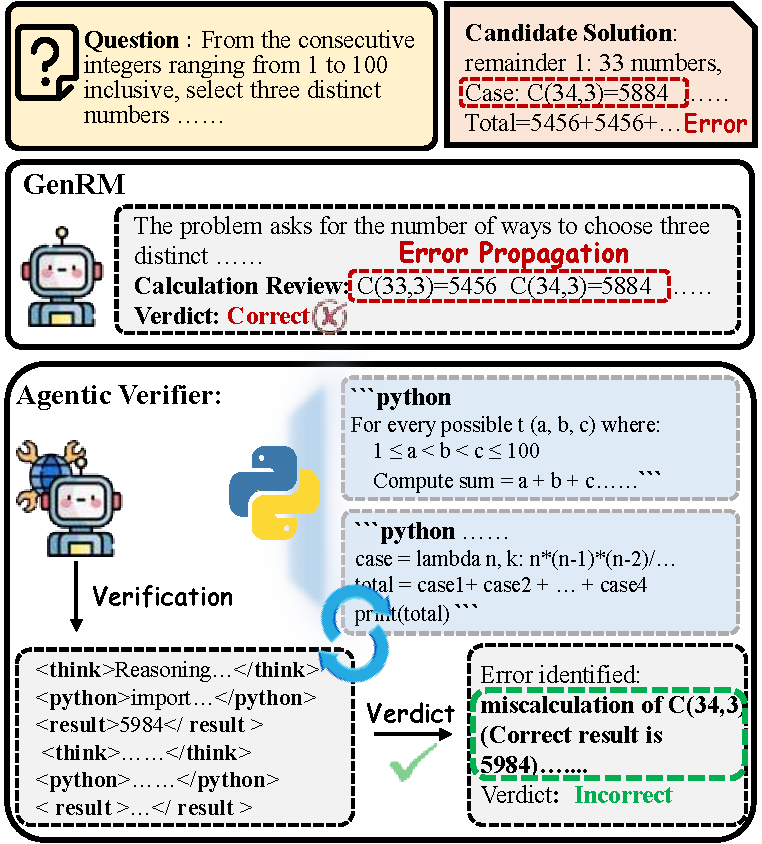
\includegraphics[width=0.95\columnwidth]{fig/Intro.pdf}
\caption{
Agentic Verifier 与 GenRM 的对比：GenRM 会受到错误传播影响并被错误解答误导，而 Agentic Verifier 借助外部依据开展严格核验。
}
\label{fig:Intro}
\vspace{-6mm}
\end{figure}

OpenAI 和 Google 在国际数学奥林匹克竞赛中取得的里程碑式进展~\citep{OAI:2025:TwitterIMO, Google:2025:GoogleIMO}，凸显了 Gemini-3、DeepSeek-Math-V2 等推理模型的迅速崛起~\citep{Shao:2025:deepseekmathv2}。
为了继续拓展 LLM 的能力边界，扩展推理时计算量已经成为主流趋势~\citep{Niklas:2025:s1, huang:2025:GeminiPipline, chen:2025:SeedProver}。无论采用并行方法（如 Best-of-$N$）还是顺序精炼，测试时扩展（TTS）的成效从根本上都依赖奖励模型，也就是验证器；它如同搜索过程的关键指南针，负责引导搜索并辨别解答质量。

\par
现有奖励模型以结果级奖励模型（ORM，\citealp{zhong2025comprehensivesurveyrewardmodels,wang2024secretsrlhflargelanguage,Zhang:2025:CRM}）和过程级奖励模型（PRM，\citealp{zhang2025lessonsdevelopingprocessreward,chen2025better,Lightman:2024:MATH500, cui2025processreinforcementimplicitrewards}）为代表，只输出标量，缺乏可解释性。
尽管近期工作开始用下一 token 预测目标训练生成式奖励模型（GenRM，\citealp{Mahan:2025:GRM,Zhang:2025:GenerativeVerifiers,Chen:2025:RM-R1,Liu:2025:DeepseekGRM}），但这类方法通常只通过单轮推理评估候选解答。具体而言，如图~\ref{fig:Intro} 所示，这一主流范式存在两个关键局限：
(1)~\textbf{错误传播}。LLM 大多基于正确或近乎正确的解答训练，因此面对有缺陷的解答时难以作出正确判定，很容易被表面合理、实际错误的答案误导~\citep{Zhang:2025:GenerativeVerifiers}。（2）~\textbf{缺少外部依据}。验证器往往难以处理计算密集型或知识密集型领域；如果不接入符号求解器或外部工具~\citep{Dong:2025:AEPO,Feng:2025:ReTool,Dong:2025:ToolStar}，就容易产生幻觉，导致性能不稳定。
这些局限表明，奖励建模需要转向一种把多轮推理与外部工具结合起来的智能体式新范式。

\par
为弥补这一缺口，我们提出 \textbf{Agentic Verifier}，一个模拟人类严谨核验过程的多智能体框架。受数学证明策略启发，Agentic Verifier 协调两个专门化智能体：前向智能体和反向智能体。
前向智能体沿着从前提到结论的逻辑流进行充分性核验；反向智能体则检查解答是否确实受题目约束支撑，从而开展必要性核验。
两个智能体都具备多轮推理和工具增强验证能力：它们可以反复把复杂解答拆成可验证的子步骤，并调用代码解释器等外部工具完成数值计算。
这种协作机制能够开展全面核验，主动识别直接错误或缺乏依据的内容，从而给出可靠判定。

\par
为解决多智能体系统训练固有的难题，我们提出 \textbf{AgentV-RL}，把这种多智能体能力蒸馏到单一模型中。
该方案包含一个自动生成验证轨迹并实施质量控制的端到端合成数据引擎，以及一个释放推理潜力的两阶段训练流程。
合成引擎自动构造覆盖广泛逻辑与计算挑战的验证轨迹，既缓解了数据稀缺，也确保困难推理模式得到全面覆盖。
在此基础上，我们先进行拒绝采样微调，再进行强化学习，以两阶段训练赋予验证器多轮、长时程、工具集成式推理能力。

\par
最后，我们在广泛设置下开展了全面实验，以检验 Agentic Verifier 的有效性。
在并行 TTS（即 BoN，Best-of-N）中，我们的 Agentic Verifier 在数学任务上超过闭源推理模型和现成的 BT-RM。
尤其值得注意的是，我们的 4B 版本持续优于参数量大十余倍的结果奖励模型 INF-ORM-Llama3.1-70B~\citep{INF_ORM_Llama3.1_70B}。
在顺序 TTS 中，Agentic Verifier 可以充当有效的批判模型，提供有价值的反馈来帮助修正求解器的缺陷。第~\ref{sec:exp} 节的深入分析验证了其有效性及其对求解器性能的提升。总体而言，本文的主要贡献如下：
\begin{itemize}[leftmargin=*]
\item 我们提出奖励建模的智能体式范式 \textbf{Agentic Verifier}，通过编排两个专门化智能体，主动找出貌似合理的解答中的缺陷。
\item 我们提出可扩展方案 \textbf{AgentV-RL}，将多智能体能力蒸馏到单一 LLM 中，使验证器具备多轮、长时程、工具集成式推理能力。
\item 实证结果证明了所提方法的有效性。值得注意的是，我们的 4B 版本超过当前最先进的 ORM，最高提升达 25.2\%。
\end{itemize}

\begin{figure*}[t]
\centering
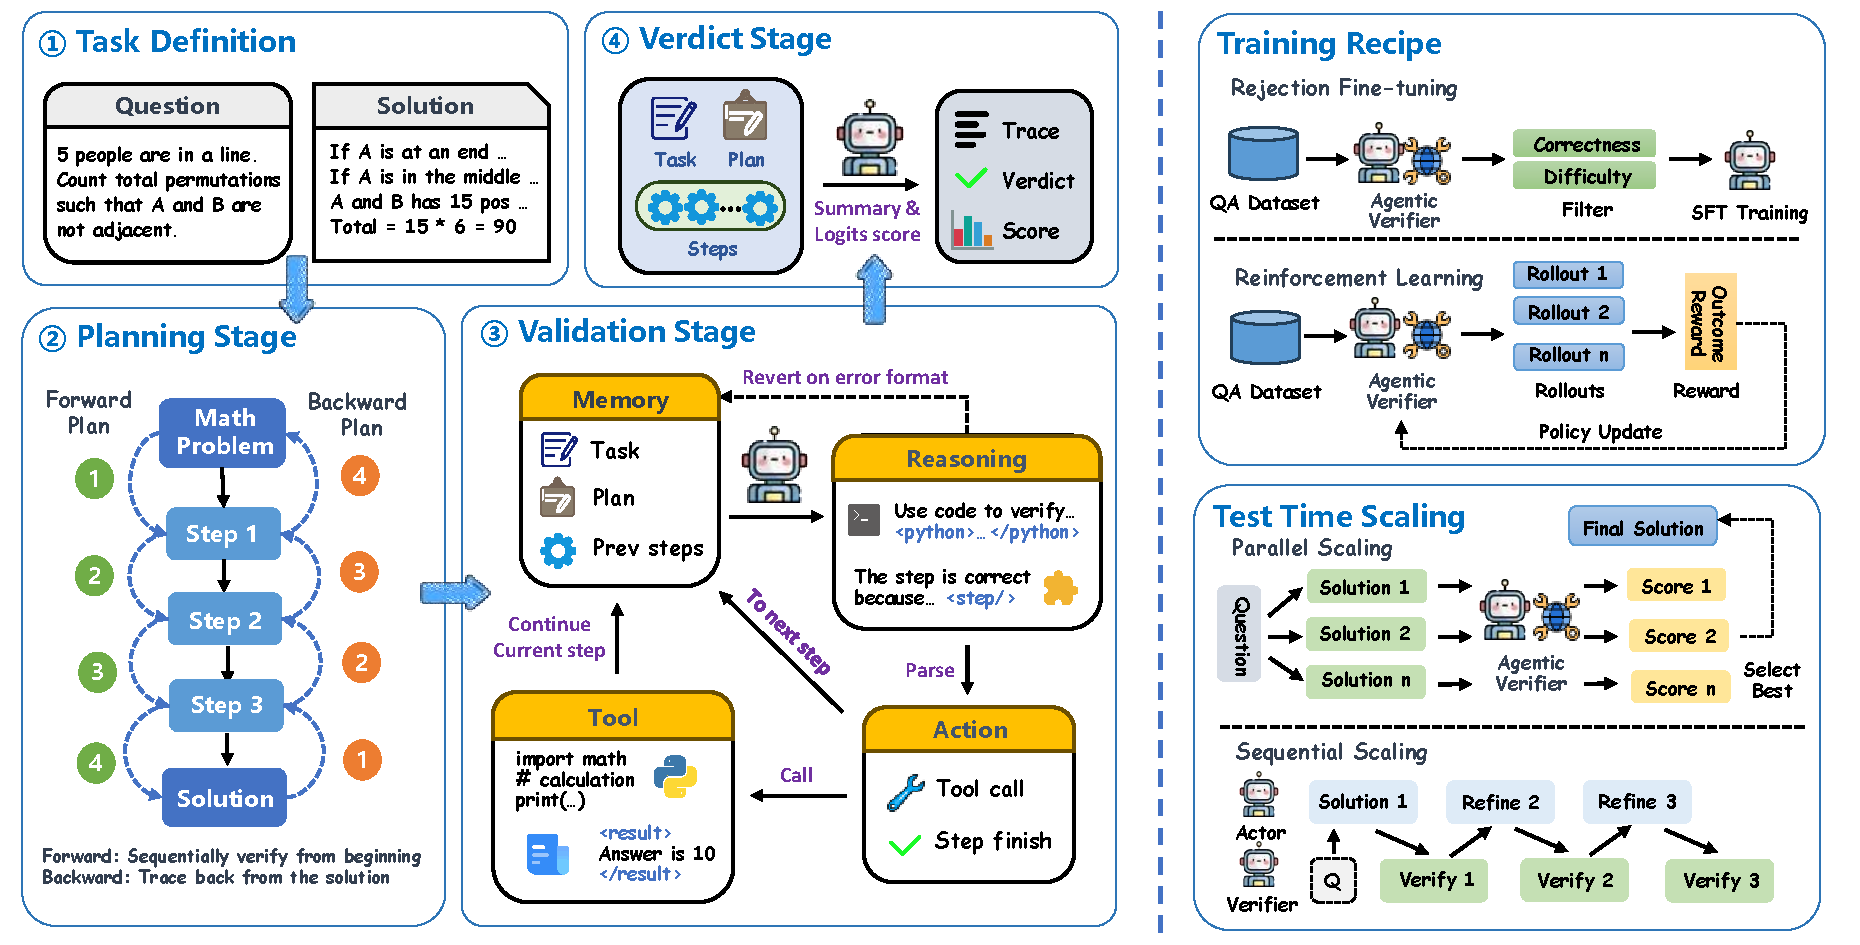
\includegraphics[width=\linewidth]{fig/Framework-full.pdf} 
\caption {
\textbf{Agentic Verifier 架构概览。}
Agentic Verifier 协调前向与反向智能体，结合多轮推理和工具增强验证，获得可靠的核验结果。
}
\label{fig:Agentic_Verifier}
\vspace{-4mm}
\end{figure*}

\section{相关工作}

\paragraph{奖励模型（RM）。}
奖励模型在使大语言模型（LLM）与人类偏好对齐的过程中发挥关键作用。
传统结果级奖励模型根据偏好排序，为完整回答赋予标量奖励~\citep{zhong2025comprehensivesurveyrewardmodels,wang2024secretsrlhflargelanguage}。
为缓解监督稀疏的限制，过程奖励模型通过监督中间步骤提供密集信号~\citep{zhang2025lessonsdevelopingprocessreward,chen2025better,Lightman:2024:MATH500,cui2025processreinforcementimplicitrewards}。
近期工作开始探索生成式奖励模型（GenRM）：它把奖励建模重新表述为下一 token 预测，并生成自然语言反馈~\citep{mahan2024GRM,chen2025judgelrm,zhang2024generative-verifiers,li2025genRMs}。
在这一范式之上，基于量规的 GenRM 会动态构造任务专用量规，并围绕评估标准展开推理~\citep{guo2025critiq,liu2025inference-time-scaling, Chen:2025:RM-R1,guo2025reward-reasoning-model}。
与此同时，还有一些方法在 LLM-as-Judge 框架下用工具增强奖励模型~\citep{Li:2024:ToolRM,Xu:2025:LLMJudgeTIR,peng2025agenticrewardmodeling}。
然而，现有方法要么没有把工具执行紧密嵌入推理过程，要么无法提供测试时扩展（TTS）所需的逐样本反馈。
相比之下，本文把验证重新表述为智能体式多轮过程，从而支持测试时探索和可靠评估。

\paragraph{测试时扩展与验证器。}
近期研究表明，扩展推理时计算可以显著增强 LLM 推理，测试时扩展（TTS）也已经成为并行选择和顺序精炼的通用范式~\cite{muennighoff2025s1}。在这一设置中，基于批判的方法利用辅助模型，在测试时指导求解器纠错和自我改进~\cite{xi2024enhancing}；更新的研究还表明，奖励模型和过程验证器本身也能从额外的推理时计算中获益~\cite{liu2025inference,khalifa2025process}。本文与这一研究方向密切相关，但区别在于，我们将验证建模成双向、多轮、工具增强的过程，使其能够在并行和顺序 TTS 中同时开展充分性与必要性核验。

\section{方法}
\label{sec:method}
本文关注数学任务中求解器与验证器之间的交互式 TTS 行为。求解器负责解题，验证器则为生成的解答链提供监督反馈。

\paragraph{并行扩展。} Best-of-N（BoN）已经成为常用的并行采样策略，它利用验证器选择高质量解答~\citep{Gui:2024:BoNAlignment,Kang:2025:ScalableBoN}。具体而言，对于给定输入 $x$，求解器采样 $k$ 个候选解答，记为 $\{y^{(j)}\}_{j=1}^{k}$。随后，验证器 $\pi_{\psi}$ 评估这些候选解答，并生成验证依据 $f$ 来判断其正确性。最后，选择在 $\pi_{\psi}$ 下置信分数最高的解答。该分数定义为验证批判 $f$ 中 \true\ token 的概率，计算如下：
\begin{align}
l(x, y^{(j)})&=\pi_{\psi}(\text{\true} \mid x, y^{(j)}, f^{(j)},\mathbf{I}) \nonumber \\
f^{(j)}\sim &\pi_{\psi}(x,y^{(j)}, \mathbf{I}),
\label{eq:boN}
\end{align}
其中，$\mathbf{I}$ 是指令：“求解过程是否正确？”（\raisebox{0.2ex}{\true}/\raisebox{0.2ex}{\false}）。

\paragraph{顺序扩展。} 给定问题 $x$ 和初始解答 $y_0$，验证器分析求解过程并给出监督性批判，即 $f_{0} \sim \pi_{\psi}(x, y_{0})$。求解器随后接收这一反馈，把解答精炼为 $y_1$。这一精炼循环可以重复多轮，直至得到正确答案或满足停止条件，形式化表示为
\begin{equation}
y_{t} \sim \pi_{\theta}(x, y_{0}, f_{0},\ldots,y_{t-1},f_{t-1}).
\label{eq:refine}
\end{equation}

\subsection{Agentic Verifier}
如图~\ref{fig:Intro} 所示，主流 GenRM 受限于单轮推理，容易发生错误传播和注意力漂移，因而难以实现可靠验证。
如图~\ref{fig:Agentic_Verifier} 所示，我们提出 \textbf{Agentic Verifier}，协调互补的前向与反向智能体：前者从前提向结论追踪解答，后者则依据前提重新审视结论。
两个智能体都支持多轮推理和工具增强验证：它们可以反复把复杂解答分解为可验证的子步骤，并调用代码等外部工具完成数值计算。
完整细节见附录~\ref{sec:appendix_ours_prompts}。

\begin{figure*}[t]
\centering
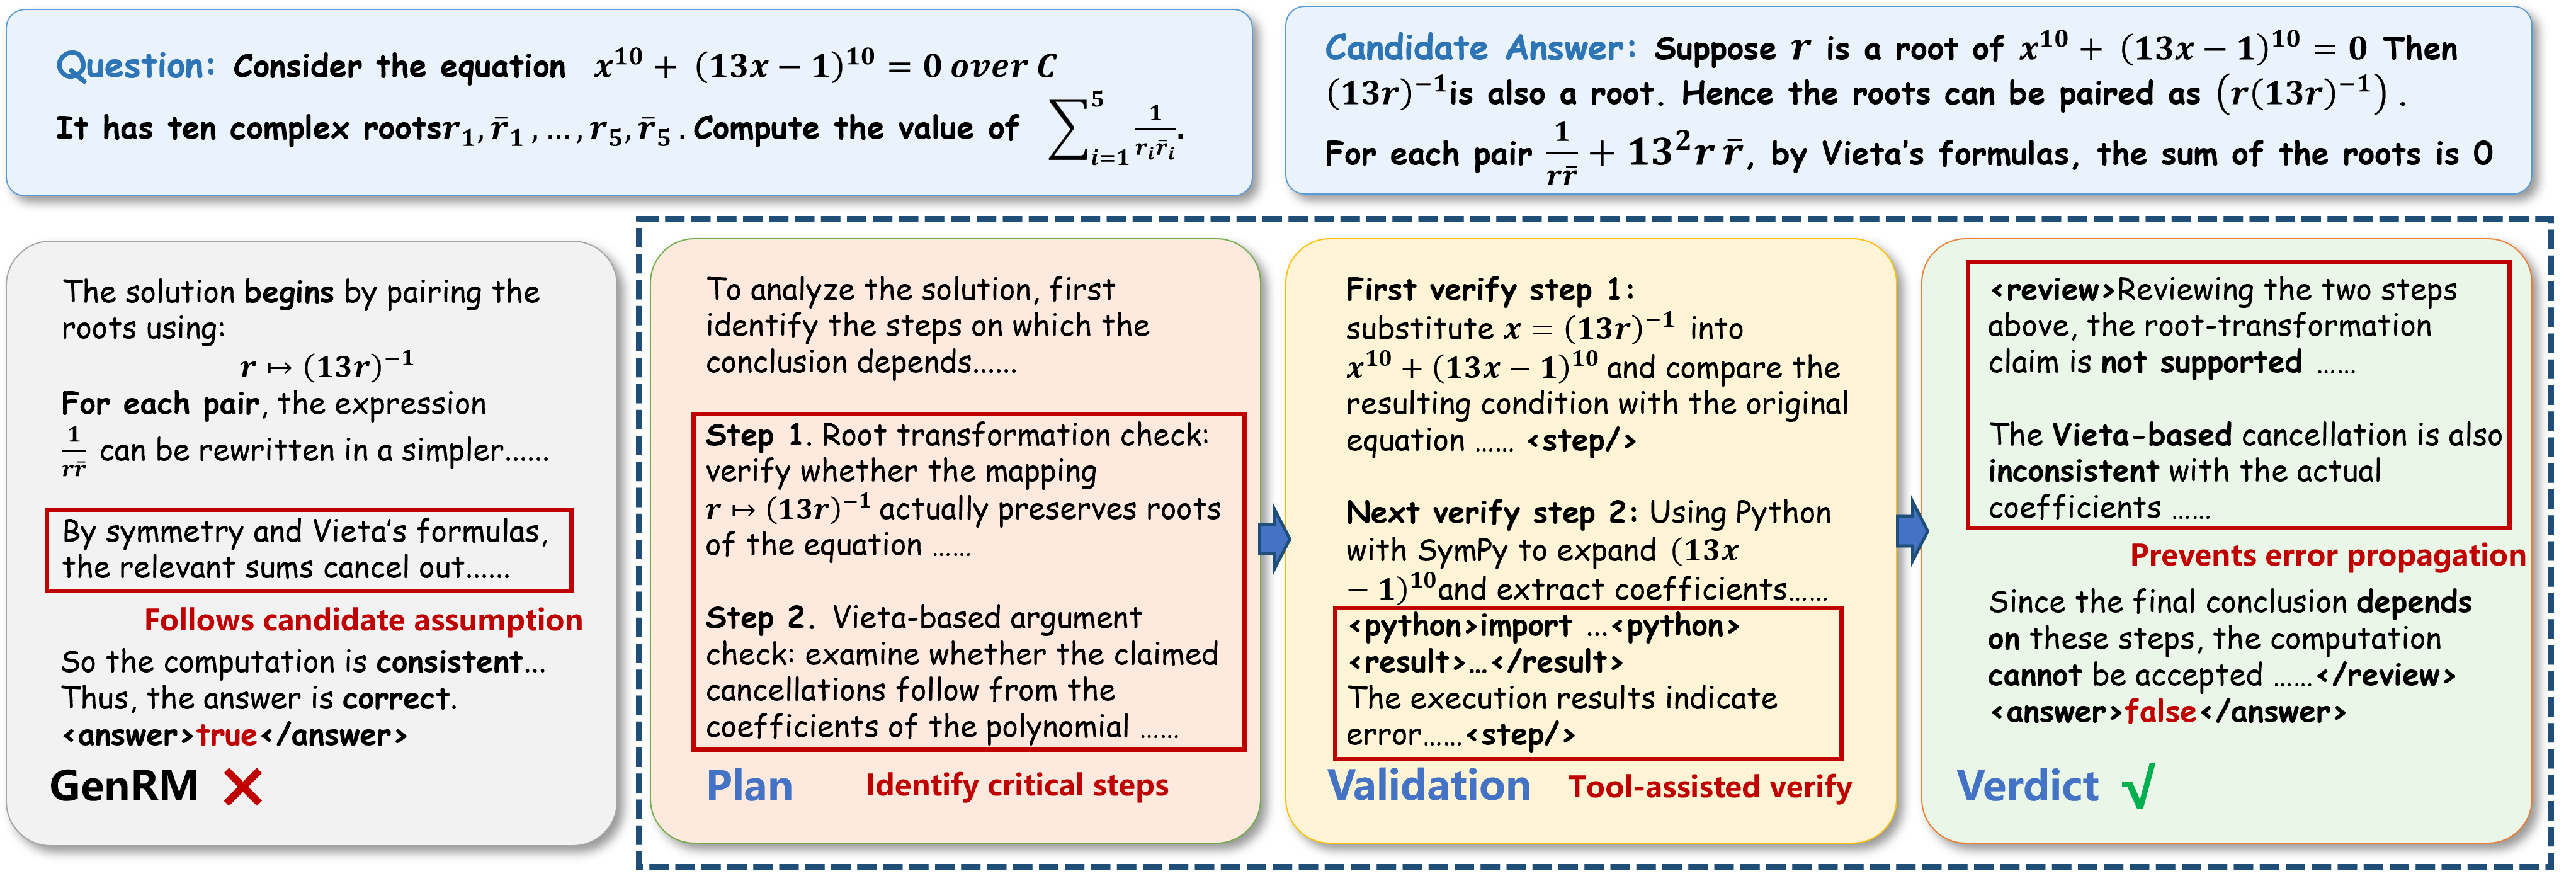
\includegraphics[width=\linewidth]{fig/1226/case_study.png}
\caption{
\textbf{GenRM 与 Agentic Verifier 的案例对比。}
该示例凸显了 GenRM 的错误传播问题，而我们的方法能够得到正确判定。更多示例见附录~\ref{sec:appendix_case}。}
\label{fig:case_study}
\vspace{-5mm}
\end{figure*}
\subsection{任务定义}
形式化地，给定 $\mathcal{D}=\left\{\left(x, g\right)\right\}$，其中 $x$ 是问题，$g$ 是标准答案。求解器 $\pi_{\theta}$ 以自回归方式生成解答 $y \sim \pi_{\theta}(\cdot| x)$；该解答由逐步的思维链（CoT）推理过程和最终答案 $\tilde{y}$ 构成。
遵循~\citet{Xi:20254:Critique, Zhang:2025:GenerativeVerifiers}，我们研究两种常见的测试时扩展范式：并行扩展和顺序扩展。

\paragraph{前向智能体。}
前向智能体从题目前提出发，沿解题路径顺序追踪，检查解答中的每一步是否正确，并验证前一步是否构成后续推导的充分条件。
为激发智能体能力，我们采用图~\ref{fig:case_study} 所示的“规划--验证--判定”策略：
\begin{itemize}[leftmargin=*]
\item \textbf{规划。} 此阶段旨在把过于复杂的推理解答分解成一系列原子化、可验证的子步骤 $\Pi = \{v_1, v_2, \dots, v_n\}$。智能体制定一份明确计划，规定下一阶段要遵循的逻辑流程。该计划包含具体检查点和必要计算，为整个验证过程建立结构化模板。

\item \textbf{验证。} 接收计划 $\Pi$ 后，智能体检查每个原子步骤 $v_i$ 的正确性，确保 $v_{i-1}$ 与 $v_i$ 之间具有逻辑充分性。
智能体可以调用 Python 解释器，并把执行结果纳入推理链。
遵循~\citet{yao2022react}，该过程包含多轮“思考--动作--观察”：
\begin{equation}
\mathcal{H} = (s_0,a_0,o_0,s_1,\ldots,s_{t},a_{t},o_{t})
\end{equation}
其中，智能体表述思考 $s$，执行动作 $a$（Python），并接收解释器返回的观察 $o$。调用 Python 的动作片段用 \actionl\ 和 \actionr\ 包围；更多细节见附录~\ref{sec:appendix_steps_prompt}。

\item \textbf{判定。} 在最后阶段，智能体从局部、逐步分析转向全局、整体评估。它汇总前一阶段收集的证据，对解答是否正确作出明确判断。输出是用 \answerl\ 和 \answerr\ 包围的严格二分类结果（\raisebox{0.2ex}{\true}/\raisebox{0.2ex}{\false}）；我们采用 \true\ 的 logit 作为判定置信信号。
\end{itemize}

\paragraph{反向智能体。}
反向智能体旨在识别前向智能体可能漏掉的错误，例如解答表面逻辑通顺，实际上却不满足题目约束，或省略了必要证明。它从最终答案反向推理到题目陈述，以验证解答的必要性。
反向智能体同样遵循“规划--验证--判定”流程，把解答分解为可反向核验的步骤，并系统检查所有必需条件是否满足。
我们汇总前向与反向智能体的结果，得到双向且可靠的评估；具体方法见附录~\ref{sec:appendix_aggregation}。

    
    

    

\begin{table*}[th]
\centering
\vspace{-2mm}
\resizebox{\textwidth}{!}{
\begin{tabular}{l|cccccccccccc}
\toprule[1.6pt]
    \textbf{模型} & \multicolumn{3}{c|}{\textbf{MATH500}} & \multicolumn{3}{c|}{\textbf{GSM8K}} & \multicolumn{3}{c|}{\textbf{Gaokao2023}} & \multicolumn{3}{c}{\textbf{AIME24}}  \\ \cmidrule{1-13}
    \textbf{BoN} & \textit{\textbf{@32}} & \textit{\textbf{@64}} & 
    \multicolumn{1}{c|}{\textit{\textbf{@128}}} & \textit{\textbf{@32}} 
    & \textit{\textbf{@64}} & \multicolumn{1}{c|}{\textit{\textbf{@128}}}  & \textit{\textbf{@32}}  & \textit{\textbf{@64}}  & \multicolumn{1}{c|}{\textit{\textbf{@128}}}  &  \textit{\textbf{@32}} & \textit{\textbf{@64}}  &  \textit{\textbf{@128}}   \\ 
    \midrule
        \multicolumn{13}{c}{\textit{\textbf{文本推理 LLM}}} \\
    \midrule
    Qwen2.5-7B-Instruct
& 53.0 & 50.4 & 51.0
& 85.5 & 85.7 & 83.9
& 40.8 & 42.3 & 41.3
& 30.0 & \underline{26.7} & \underline{33.3} \\

Llama3.1-8B-Instruct
& 46.7 & 48.0 & 45.2
& 81.5 & 80.1 & 81.7
& 34.5 & 35.6 & 35.6
& 30.0 & \textbf{30.0} & 30.0 \\

Qwen3-4B-Think
& \textbf{70.0} & \textbf{72.6} & \textbf{72.4}
& \textbf{92.3} & \textbf{91.2} & \textbf{92.2}
& \textbf{52.2} & \textbf{51.4} & \textbf{51.9}
& \textbf{40.0} & \textbf{30.0} & \textbf{36.7} \\

DS-Distill-14B
& \underline{66.2} & \underline{69.6} & \underline{69.4}
& \underline{90.1} & \underline{88.9} & \underline{89.8}
& \underline{48.3} & \underline{49.1} & \underline{48.6}
& \underline{33.3} & \underline{26.7} & \underline{36.7} \\

Mistral-Small-24B-Instruct
& 52.2 & 51.0 & 51.8
& 85.4 & 85.5 & 85.9
& 39.0 & 38.4 & 40.0
& 30.0 & \textbf{30.0} & \textbf{36.7} \\
    \specialrule{1pt}{0.4ex}{0.4ex}

    \multicolumn{13}{c}{\textit{\textbf{结果级 RM}}} \\
    \midrule

    GRM-Gemma-2B
& 45.6 & 48.8 & 46.6
& 77.9 & 75.5 & 73.4
& 33.5 & 31.9 & 33.2
& {33.3} & 26.7 & 30.0 \\

Skywork-V2-Llama-8B
& \underline{54.4} & \underline{55.2} & \underline{53.8}
& 87.5 & 87.3 & {87.6}
& \textbf{41.6} & 37.4 & {39.7}
& 30.0 & \underline{33.3} & \underline{36.7} \\

InternLM2-20B-RM
& {54.0} & {52.2} & {53.6}
& \underline{89.5} & \underline{89.6} & \underline{89.8}
& \textbf{41.6} & \textbf{42.9} & \underline{43.9}
& \underline{36.7} & \textbf{36.7} & {40.0} \\

INF-ORM-Llama3.1-70B
& \textbf{54.6} & \textbf{56.4} & \textbf{55.4}
& \textbf{91.2} & \textbf{90.8} & \textbf{91.5}
& \underline{40.8} & \underline{42.6} & \textbf{44.4}
& \textbf{40.0} & \textbf{36.7} & \textbf{40.0} \\

Starling-RM-34B
& 50.0 & 52.0 & 50.8
& {88.4} & {87.6} & 86.3
& 40.5 & {39.7} & 39.0
& 26.7 & 33.0 & \underline{36.7} \\
    
    
    \specialrule{1pt}{0.4ex}{0.4ex}

    \multicolumn{13}{c}{\textit{\textbf{过程级 RM}}} \\
    \midrule
    Qwen2.5-Math-PRM-7B
& \underline{65.2} & \textbf{69.4} & \textbf{70.2}
& \textbf{94.5} & \textbf{94.7} & \textbf{95.4}
& \textbf{50.9} & \textbf{51.4} & \textbf{54.3}
& \textbf{43.3} & \textbf{43.3} & \textbf{46.7} \\

Math-Shepherd-Mistral-7B-PRM
& \textbf{66.6} & \underline{66.6} & \underline{66.6}
& {90.0} & {89.2} & {89.6}
& {43.1} & {41.4} & {39.3}
& \textbf{30.0} & {36.7} & {30.0} \\

EurusPRM-Stage1
& 38.8 & 36.0 & 33.8
& 70.0 & 66.3 & 62.5
& 33.2 & 29.1 & 26.8
& 20.0 & 23.3 & 26.7 \\

EurusPRM-Stage2
& 36.0 & 31.8 & 31.0
& 66.0 & 62.1 & 57.5
& 29.1 & 26.5 & 25.7
& 16.7 & 20.0 & 23.3 \\

Skywork-PRM
& {61.6} & {66.2} & {65.6}
& \underline{92.5} & \underline{92.7} & \underline{93.4}
& \underline{46.0} & \underline{47.0} & \underline{46.8}
& {23.3} & \textbf{40.0} & \textbf{33.3} \\

    \specialrule{1pt}{0.4ex}{0.4ex} 
    \multicolumn{13}{c}{\textit{\textbf{本文方法}}} \\
    \midrule
    Agentic-Verifier-Llama3-8B
    & 59.6 & 60.8 & 60.6
    & 90.8 & 91.2 & 90.7
    & 45.5 & 47.3 & 47.0
    & 30.0 & 33.3 & 40.0 \\
    
    Agentic-Verifier-Qwen3-4B
    & \textbf{73.8} & \textbf{76.2} & \textbf{79.0}
    & \textbf{93.0} & \textbf{92.6} & \textbf{93.3}
    & \textbf{54.5} & \textbf{55.1} & \textbf{57.4}
    & \textbf{46.7} & \textbf{50.0} & \textbf{53.3} \\

    \bottomrule[1.6pt]
\end{tabular}}
\caption{
\textbf{Best-of-N 采样在 GSM8K、MATH500、Gaokao2023 和 AIME24 上的性能（\%）。} 每个类别中的最佳结果以粗体标出，次佳结果加下划线。
}
\label{Tab:Main_Exp_BoN}
\vspace{-5mm}
\end{table*}

\subsection{AgentV-RL}
上述双向设计为识别候选解答中的缺陷提供了有效的多智能体框架。
此外，要把多智能体能力蒸馏进单一 LLM，还需要专门的训练方案。
本节提出 \textbf{AgentV-RL}，一个由合成数据引擎和两阶段训练流程组成的可扩展方案。

\subsubsection{合成轨迹采样}
为了让验证器初步掌握工具集成式验证，我们设计了一条合成数据流水线，用于获得高质量多轮轨迹。
具体而言，我们筛选 Polaris~\citep{An:2025:polaris}、DeepScaleR-40K~\citep{Luo:2025:deepscaler} 和 AReaL-boba-106k~\citep{Mei:2025:AReaL} 等高质量公开数据集，整理训练数据。
为保证合成数据的多样性，我们为每个问题采样 $k$ 个解答（取 $k=8$），并过滤掉 $k$ 个解答全对或全错的问题。
由此得到包含候选解答的初始数据集 $\mathcal{D}_{init} = \{x, y, l\}$，其中 $l \in \{\text{\raisebox{0.2ex}{\true}} / \text{\raisebox{0.2ex}{\false}}\}$ 表示解答 $y$ 是否正确。

\par
基于 $\mathcal{D}_{init}$，我们使用 LLM 自动生成工具增强的验证轨迹。
具体而言，LLM 扮演前向或反向智能体，生成以最终判定 $\tilde{l}$ 结束的验证轨迹 $\mathcal{H}$。
为控制质量，我们只保留预测判定 $\tilde{l}$ 与标准标签 $l$ 一致的轨迹。
最终得到同时包含正、负验证样例的数据集 $\mathcal{D}_{\text{sft}}$：
\begin{equation}
\mathcal{D}_{\text {sft }}=\left\{\left(x, y^{+}, \mathcal{H}^{+}\right)\right\} \cup\left\{\left(x, y^{-}, \mathcal{H}^{-}
\right)\right\},
\end{equation}
其中，前一项表示被判定为 \true\ 的正轨迹 $\mathcal{H}^{+}$，后一项表示被判定为 \false\ 的负轨迹 $\mathcal{H}^{-}$。

\subsubsection{拒绝采样微调}
利用合成数据集 $\mathcal{D}_{\text{sft}}$，我们开展监督微调（SFT），使验证器掌握智能体式能力。此阶段旨在让模型行为与多轮决策过程对齐。

\par
核心目标是鼓励验证器复现逐步推理和有效的工具交互。形式化地，对于每个数据点 $(x, y, \mathcal{H})$，$x$ 是问题，$y$ 是候选解答，$\mathcal{H}=(\tau_0,\tau_1,\ldots,\tau_n)$ 是标注后的验证轨迹，其中每个 $\tau_i \in \{s_i,a_i,o_i\}$；我们优化如下损失：
\begin{equation}
\mathcal{L} = - \mathbb{E}_{\tau \sim \mathcal{H}} \left[\sum_{i=1}^{|\mathcal{H}|} \mathbb{I}\left[\tau_i \neq o_i \right] \cdot \log \pi_\theta\left(\tau_i \mid \mathcal{H}_{<i}\right)\right]
\end{equation}

\subsubsection{强化学习}
为了进一步释放 Agentic Verifier 的推理潜力并激励自主探索，我们在训练方案中引入组相对策略优化（GRPO）。在 SFT 之后，此阶段优化推理模式，以实现多轮、长时程、工具集成式推理。
具体而言，对于每个问题--解答对，我们从验证器 $\pi_{\psi}$ 采样一组候选轨迹：
\begin{equation}
\left\{\mathcal{H}_i\right\}_{i=1}^G \sim \pi_{\psi}(\cdot \mid x, y, \mathbf{I}),
\end{equation}
其中，$\mathbf{I}$ 表示具体的指令提示。在实验中，我们采用混合采样策略，让 $\pi_{\psi}$ 分别扮演前向或反向智能体，从而对两个视角进行均衡优化。

\section{实验}
\label{sec:exp}
\begin{table*}[t]
    \centering
    \vspace{-2mm}
    \resizebox{\textwidth}{!}{
    \begin{tabular}{l|cccccccccccc}
    \toprule
        \textbf{验证器} & \multicolumn{3}{c}{\textbf{MATH500}} & \multicolumn{3}{c}{\textbf{GSM8K}} & \multicolumn{3}{c}{\textbf{Gaokao2023}} & \multicolumn{3}{c}{\textbf{AIME24}}  \\ \cmidrule{1-13}

        \textbf{指标} & \textit{\textbf{准确率}} & \textit{\textbf{$\Delta_\uparrow$}} & \textit{\textbf{$\Delta_\downarrow$}} & \textit{\textbf{准确率}} & \textit{\textbf{$\Delta_\uparrow$}} & \textit{\textbf{$\Delta_\downarrow$}}
        & \textit{\textbf{准确率}} & \textit{\textbf{$\Delta_\uparrow$}} & \textit{\textbf{$\Delta_\downarrow$}}
        & \textit{\textbf{准确率}} & \textit{\textbf{$\Delta_\uparrow$}} & \textit{\textbf{$\Delta_\downarrow$}}
        \\ 
        \midrule
            \multicolumn{13}{c}{\textit{\textbf{第 1 轮}}} \\
        \midrule
        Qwen2.5-7B-Instruct
& 60.4 & 14.0 & 0.6
& 85.9 & 5.9 & 0.6
& 47.0 & 12.7 & 2.9
& 13.3 & 0.0 & 0.0 \\

Llama3.1-8B-Instruct
& 54.6 & 11.0 & 3.4
& 84.1 & 4.6 & 1.1
& 44.9 & 10.7 & 2.9
& 13.3 & 0.0 & 0.0 \\

Qwen3-4B-Think
& 80.0 & 33.8 & 0.8
& 90.9 & 11.1 & 0.9
& 64.9 & 31.2 & 3.4
& 16.7 & 3.3 & 0.0 \\

DS-Distill-14B
& \underline{83.0} & 37.4 & 1.4
& \underline{92.0} & 12.1 & 0.8
& \underline{67.0} & 32.5 & 2.6
& \underline{23.3} & 10.0 & 0.0 \\

Mistral-Small-24B-Instruct
& 61.4 & 15.6 & 1.2
& 88.4 & 8.5 & 0.8
& 49.1 & 15.6 & 3.6
& 13.3 & 0.0 & 0.0 \\

Agentic-Verifier-Qwen3-4B
& \textbf{84.2} & 41.6 & 0.6
& \textbf{94.6} & 14.5 & 0.5
& \textbf{75.6} & 40.3 & 1.8
& \textbf{40.0} & 26.7 & 3.3 \\
        \midrule
            \multicolumn{13}{c}{\textit{\textbf{第 2 轮}}} \\
        \midrule
       Qwen2.5-7B-Instruct
& 64.8 & 6.2 & 1.8
& 87.4 & 3.3 & 1.9
& 49.9 & 5.2 & 2.3
& 6.7 & 0.0 & 6.7 \\

Llama3.1-8B-Instruct
& 58.4 & 6.0 & 2.2
& 82.8 & 3.3 & 4.6
& 48.1 & 5.2 & 2.1
& 10.0 & 0.0 & 3.3 \\

Qwen3-4B-Think
& 84.6 & 6.0 & 1.4
& 92.2 & 2.4 & 1.1
& 69.1 & 5.5 & 1.3
& 23.3 & 6.7 & 3.3 \\

DS-Distill-14B
& \underline{87.4} & 5.8 & 1.4
& \underline{92.7} & 2.4 & 1.7
& \underline{70.1} & 4.7 & 1.6
& \underline{26.7} & 3.3 & 0.0 \\

Mistral-Small-24B-Instruct
& 66.4 & 5.8 & 0.8
& 90.0 & 2.7 & 1.1
& 52.7 & 4.9 & 1.3
& 13.3 & 0.0 & 0.0 \\

Agentic-Verifier-Qwen3-4B
& \textbf{89.2} & 2.4 & 1.2
& \textbf{94.1} & 0.4 & 0.9
& \textbf{76.6} & 3.4 & 2.3
& \textbf{33.3} & 0.0 & 6.7 \\
        \midrule
            \multicolumn{13}{c}{\textit{\textbf{第 3 轮}}} \\
        \midrule
        Qwen2.5-7B-Instruct
& 66.0 & 4.2 & 3.0
& 87.5 & 2.96 & 2.8
& 52.2 & 3.64 & 1.3
& 10.0 & 6.7 & 3.3 \\

Llama3.1-8B-Instruct
& 58.8 & 4.0 & 3.6
& 82.8 & 3.3 & 3.3
& 47.0 & 1.3 & 2.3
& 6.0 & 0.0 & 3.00 \\

Qwen3-4B-Think
& 84.8 & 2.4 & 2.2
& 92.0 & 1.2 & 1.4
& 69.6 & 2.3 & 1.6
& 26.0 & 6.7 & 3.0 \\

DS-Distill-14B
& \underline{85.8} & 2.2 & 3.8
& \underline{93.4} & 1.8 & 1.1
& \underline{73.0} & 4.4 & 1.6
& \underline{33.0} & 6.7 & 0.0 \\

Mistral-Small-24B-Instruct
& 67.8 & 4.4 & 3.0
& \cellcolor{lightgreen1}{90.6} & 2.65 & 2.05
& 52.2 & 2.08 & 2.60
& 13.0 & 0.00 & 0.00 \\

Agentic-Verifier-Qwen3-4B
& \textbf{89.8} & 1.8 & 1.2
& \textbf{94.1} & 1.0 & 1.0
& \textbf{76.4} & 2.6 & 2.9
& \textbf{33.0} & 3.3 & 3.3 \\
        \bottomrule[1.6pt]
    \end{tabular}
    }
\caption{\textbf{不同验证器在迭代精炼中的性能对比。}
\textit{准确率}表示每轮精炼后的平均准确率；$\Delta_\uparrow$ 和 $\Delta_\downarrow$ 分别衡量相较前一轮的纠错率与退化率。
最佳结果以\textbf{粗体}标出，次佳结果\underline{加下划线}。
}
\label{Tab:Main_Exp_Refine}
\vspace{-2mm}
\end{table*}

\paragraph{可验证奖励。}
我们比较预测判定 $\tilde{l}$ 与标准标签 $l$ 是否一致，并采用二元结果级奖励：
\begin{equation}
r(\mathcal{H})= \begin{cases}1, & \text {若 } \tilde{l}=l 
 \\ -1, & \text {否则} \end{cases}
\end{equation}
遵循~\citet{Yu:2025:DAPO}，我们动态过滤奖励方差为零的轨迹组；这类样本对策略模型而言过易或过难（组内几乎全为 $+1$ 或全为 $-1$）。随后，我们在每组内计算归一化优势 $\hat{A}_{i,t}$，并用以下目标更新验证器：
\begin{align}
& \mathcal{J}_{\mathrm{GRPO}}(\psi)=\mathbb{E}_{(x,y ) \sim \mathcal{D},\left\{\mathcal{H}_i\right\}_{i=1}^G \sim \pi_{\psi_{\text {old }}}} 
\frac{1}{G}  \sum_{i=1}^G \frac{1}{\left|\mathcal{H}_i \right|} \nonumber  \\
& \sum_{t=1}^{\left| \mathcal{H}_i \right|}  
\min( r_{i, t}(\psi) \hat{A}_{i, t}, \operatorname{clip} (r_{i, t}(\psi), 1-\epsilon_{low}, 1+  \nonumber  \\
& \epsilon_{high}) \hat{A}_{i, t} ) - \beta D_{\mathrm{KL}}\left(\pi_\psi \| \pi_{\text {ref }}\right) 
\end{align}
其中，$r_{i, t}(\psi)=\frac{\pi_\psi\left(\mathcal{H}_{i} \mid x, y, \mathcal{H}_{i,<t} \right)}{\pi_{\psi_{\text {old }}}\left(\mathcal{H}_{i} \mid x, y, \mathcal{H}_{i,<t}\right)}$ 是重要性采样比率。
为降低模型记忆环境观察的风险，我们不把编译器执行结果计入损失。

\subsection{实验设置}
\paragraph{任务。}
我们从两种主流 TTS 范式评估所提方法：并行扩展和顺序扩展。前者关注 BoN，后者则让验证器迭代指导修订。
实验采用广泛使用的推理基准：GSM8K~\citep{Cobbe:2023:GSM8k}、AIME24~\citep{AIME:2024:AIME}、MATH500~\citep{Lightman:2024:MATH500} 和 Gaokao2023~\citep{Liao:2024:Gaokao2023}。

\paragraph{实现细节。}
我们使用 Qwen3-4B~\citep{Yang:2025:Qwen3} 作为基础模型。在 SFT 阶段，验证器使用第~\ref{sec:method} 节构造的 15K 条合成样本训练；随后，再使用额外 50K 条样本通过 GRPO 进一步优化。实现细节见附录~\ref{sec:appendix_impl_details}。

\paragraph{评测设置。}
对于并行扩展，我们报告不同采样轨迹数 $N$ 下的准确率：验证器为 $N$ 个候选解答打分，并选择得分最高者作为最终输出。对于顺序扩展，我们报告每轮精炼后的平均准确率，以及衡量相较前一轮纠错率和退化率的 $\Delta_\uparrow$ 与 $\Delta_\downarrow$。为确保严格可比，所有验证器变体都在同一固定候选池上评测，而且每个问题实例使用相同的初始解答。更多评测细节和基线说明见附录~\ref{sec:appendix_eval_protocol} 与附录~\ref{sec:appendix_baselines}。

\subsection{主要结果}
\captionsetup{skip=4pt}
\begin{figure*}[t]
\centering
\begin{subfigure}[t]{0.49\textwidth}
\centering
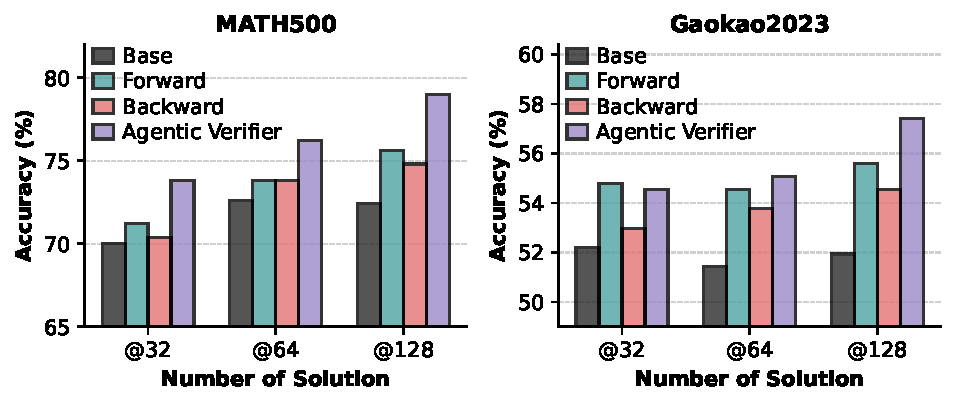
\includegraphics[width=\linewidth]{fig/1226/component_bon.pdf}
\label{fig:bon}
\end{subfigure}
\hfill
\begin{subfigure}[t]{0.49\textwidth}
\centering
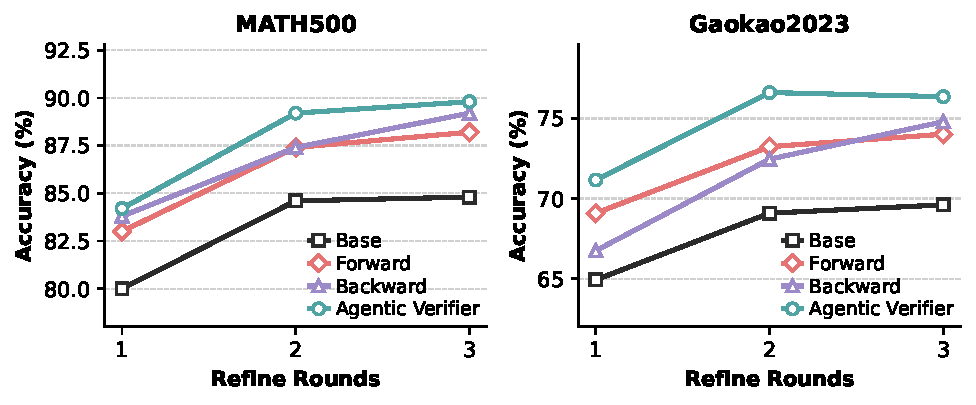
\includegraphics[width=\linewidth]{fig/1226/component_refine.pdf}
\label{fig:refine}
\end{subfigure}
\vspace{-10pt}
\caption{
\textbf{不同变体在 Best-of-N 采样（左）和验证器修订（右）上的消融实验。}
仅前向与仅反向变体都具有竞争力，而完整设计表现最佳。
}
\vspace{-5mm}
\label{fig:ablation_bon_refine_component}
\end{figure*}

\paragraph{Agentic Verifier 提升 Best-of-N 采样性能。}
表~\ref{Tab:Main_Exp_BoN} 报告了与当前先进方法对比的 BoN 性能。
我们得到以下几项关键观察：
\textit{（1）}Agentic Verifier 在所有基准上都持续表现强劲，刷新了当前最佳结果。尤其是 Agentic-Verifier-Qwen3-4B 在 MATH500 上取得最高 79.0\% 的准确率，比此前最佳结果级 RM Skywork-V2-Llama-8B 高出 25.2 个百分点。在 GSM8K、Gaokao2023 和 AIME24 上也能观察到类似趋势，我们的模型均保持明显领先。
\textit{（2）}随着 BoN 样本数 $N$ 从 32 增至 128，Agentic Verifier 的性能继续稳定提升，在 AIME24 等高难度基准上尤为明显。在 AIME24 上，4B 变体在 $N=128$ 时达到 53.3\% 的准确率，而包括更大模型在内的所有基线都明显更低。
\textit{（3）}与 Qwen3-4B、Llama-3.1-8B 等基础模型相比，我们的变体带来了大幅提升。
这些显著收益源自所提框架中的双向验证和无缝工具集成；二者使模型能够仔细审查推理链并捕捉细微错误，尤其适用于 AIME24 这类高难度基准。

\paragraph{Agentic Verifier 为迭代精炼提供有效指导。}
为评估验证器反馈的帮助程度，我们对不同验证器下的“批判--修订”策略进行了全面分析。
根据表~\ref{Tab:Main_Exp_Refine} 的结果，可以得到以下结论：
\textit{（1）}在第 1 轮中，借助 Agentic-Verifier-Qwen3-4B 的批判，求解器在 GSM8K 和 MATH500 上分别达到 94.6\% 与 84.2\% 的准确率。
$\Delta_\uparrow$（错误解答得到纠正的比例）最高达到 41.6\%，同时错误修订率 $\Delta_\downarrow$ 仅为 0.6\%。
这说明 Agentic Verifier 能给出高质量批判，帮助求解器纠正错误解答。
\textit{（2）}相比其他验证器，Agentic Verifier 收敛更快：前一至两轮精炼就能带来显著性能提升。
在后续迭代中，性能保持稳定或只轻微下降，避免了 DS-Distill-14B 等模型出现的退化。这种鲁棒性得益于智能体式多轮推理和工具增强验证机制，它们使验证器能在整个精炼过程中保持严格监督。

\subsection{分析}
\subsubsection{消融实验}
\paragraph{双向组件的有效性。}
回顾前文，Agentic Verifier 包含两个专门化智能体：前向智能体沿候选解答中从前提到结论的逻辑流进行追踪；反向智能体则从最终结论反推原始问题，验证必要性。
为评估每个智能体的独立贡献，我们在 BoN 采样和验证器修订上对两个变体进行消融对比，如图~\ref{fig:ablation_bon_refine_component} 所示：（a）仅前向智能体；（b）仅反向智能体。两个变体都取得了有竞争力的结果，但整合两个智能体的 Agentic Verifier 达到了当前最佳性能。这表明双向设计的两个目标可以相互协同，从而改善泛化能力并提高验证可靠性。

\paragraph{工具使用的有效性。}
我们观察到，即使是不使用工具的变体也已显著优于基础模型，说明除工具本身带来的收益外，Agentic Verifier 框架本身也对性能提升作出了重要贡献。引入工具后，性能会进一步提高。值得注意的是，实际工具调用量保持适中且稳定。包括消融结果和执行统计在内的详细分析见附录~\ref{sec:appendix_tool}。

\begin{figure}[t]
\centering
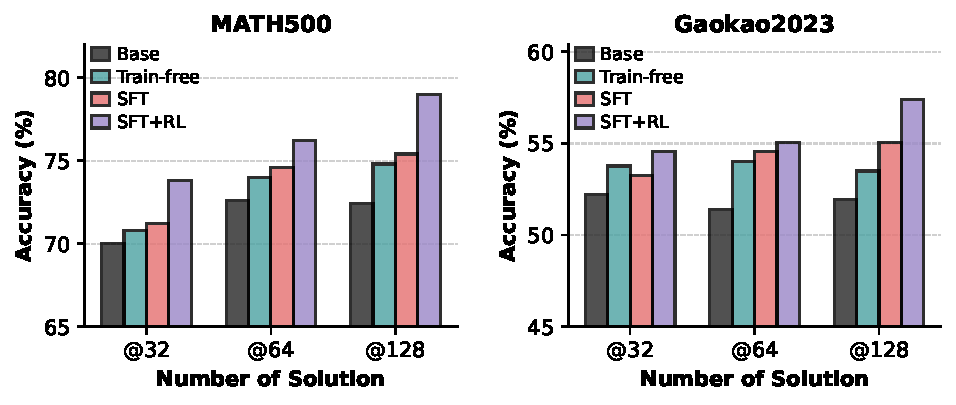
\includegraphics[width=\linewidth]{fig/1226/train_ana.pdf}
\caption{
\textbf{不同训练设计选择对 BoN 性能影响的可控实验。}
SFT+RL 设计取得最佳结果。
}
\vspace{-5mm}
\label{fig:bon_training}
\end{figure}

\paragraph{训练方案。}
我们进一步研究训练方案中的关键组成。
通过一系列可控实验，我们比较免训练、SFT 和 SFT+RL 三种配置，定量评估主要设计选择的影响。
图~\ref{fig:bon_training} 展示了实验结果，更多设置细节见附录~\ref{sec:appendix_impl_details}。
免训练变体已经取得较有竞争力的结果，在 Gaokao2023 上比基础模型最高提升 2.6 个点。
SFT 变体进一步提升了性能，验证了合成数据引擎的有效性。
最后，引入 RL 后，模型可以与环境直接交互并优化行为模式，从而进一步释放推理潜力。

\subsubsection{扩展效应}
\paragraph{扩展推理时计算。}
如式~\ref{eq:boN_TTS} 所定义，可以通过采样多条验证轨迹并聚合其分数，扩展 Agentic Verifier 的推理时计算量。
图~\ref{fig:inference_time_scaling} 表明，随着投入更多推理时计算，BoN 性能会持续提高。

\paragraph{扩展模型规模。}
我们还考察了免训练设置下扩展模型规模的效果。如表~\ref{tab:bon_model_scale} 所示，更大的模型在各项基准上始终取得更高准确率。参数量从 0.6B 扩展到 1.7B 后，Gaokao2023 性能提升 5.2 个点；扩展到 Qwen3-4B 后还会进一步提高。
这些发现表明，随着模型容量增大，模型可以持续受益于我们的智能体式框架。

\begin{figure}[t]
\centering
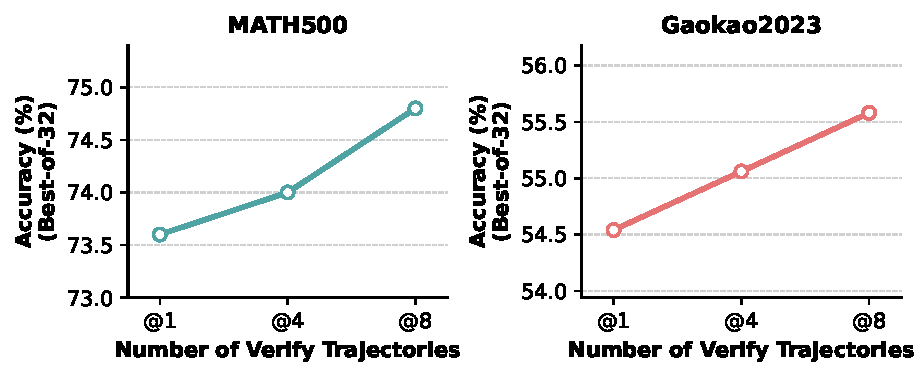
\includegraphics[width=\linewidth]{fig/1226/multi_verify.pdf}
\caption{
\textbf{扩展验证阶段的推理时计算。}
采样多条验证轨迹能够提高 BoN 准确率。
}
\label{fig:inference_time_scaling}
\vspace{-1mm}
\end{figure}

\begin{table}[t]
\centering
\small
\setlength{\tabcolsep}{6pt}
\begin{tabular}{l|ccc|ccc}
\toprule
 & \multicolumn{3}{c|}{\textbf{MATH500}} & \multicolumn{3}{c}{\textbf{Gaokao2023}} \\
\textbf{模型} & @32 & @64 & @128 & @32 & @64 & @128 \\
\midrule
0.6B & 59.8 & 63.2 & 62.2 & 43.9 & 44.9 & 43.1 \\
1.7B & 64.8 & 67.4 & 68.0 & 46.5 & 49.4 & 48.3 \\
4B   & \textbf{73.8} & \textbf{76.2} & \textbf{79.0} 
     & \textbf{54.5} & \textbf{55.1} & \textbf{57.4} \\
\bottomrule
\end{tabular}
\caption{
\textbf{使用 Qwen3 系列扩展 Agentic Verifier 的模型规模。}
更大的模型能够持续受益于所提智能体式验证框架。}
\vspace{-1mm}
\label{tab:bon_model_scale}
\end{table}

\subsubsection{泛化性能}
我们进一步在 LiveCodeBench~\cite{jain2024livecodebench} 和 HotpotQA~\cite{yang2018hotpotqa} 上评估 Agentic Verifier，以测试其在竞赛编程和多跳问答中的通用性。
Agentic-Verifier-Qwen3-4B 在两个基准上都取得最佳性能（表~\ref{tab:generalization}），证明我们的双向、工具增强范式可以泛化到更广泛的推理领域。实验细节见附录~\ref{sec:beyond_math}。

\begin{table}[t]
\centering
\small
\setlength{\tabcolsep}{10pt}
\begin{tabular}{lcc}
\toprule
模型 & LCB & HotpotQA \\
\midrule
Qwen3-4B & 57.14 & 40.00 \\
Qwen2.5-7B-Instruct & 58.29 & 40.67 \\
DS-Distill-14B & 64.57 & 52.05 \\
Mistral-Small-24B-Instruct & 50.30 & 63.00 \\
Agentic-Verifier-Qwen3-4B & \textbf{70.86} & \textbf{66.00} \\
\bottomrule
\end{tabular}
\caption{在 LiveCodeBench 和 HotpotQA 上的\textbf{泛化性能}。}
\label{tab:generalization}
\end{table}

\subsubsection{延迟分析}
\paragraph{计算开销。} 如表~\ref{tab:latency} 所示，Agentic Verifier 以更多 token 和更高延迟为代价取得最高准确率。该开销源于其多轮审议过程，而前向和反向变体可为资源受限设置提供可伸缩的权衡。基准结果是在 A100 GPU 上以 128 的批大小运行后，针对各条轨迹取平均得到的。

\begin{table}[t]
\centering
\small
\setlength{\tabcolsep}{2.6pt}
\begin{tabular}{lcccc}
\toprule
模型 & Token 数 & 轮数 & \makecell{工具\\调用数} & \makecell{时间\\（秒）} \\
\midrule
基础模型 & 2560 & 1.0 & 0.0 & 119.0 \\
前向 & 4114 & 5.7 & 0.9 & 159.1 \\
反向 & 4235 & 5.6 & 0.7 & 164.3 \\
Agentic-Verifier & 8349 & 11.3 & 1.6 & 323.4 \\
\bottomrule
\end{tabular}
\caption{
\textbf{计算成本与延迟分析。}
所有指标均在验证轨迹上取平均；延迟通过 vLLM 在单张 A100 GPU、批大小 128 的设置下测得。
}
\label{tab:latency}
\vspace{-2mm}
\end{table}

\section{结论}
本文提出 Agentic Verifier，一种利用多轮、工具增强验证的智能体式奖励建模范式。
通过编排前向与反向智能体，我们的方法能够对解答进行全面且可解释的核验。
大量实验表明，Agentic Verifier 在并行和顺序 TTS 中都带来了显著提升，并超过当前最先进的 ORM 和 PRM。这些结果表明，Agentic Verifier 是推进智能体式奖励建模的一条有前景的方向。
我们希望本工作能为奖励模型的发展提供有价值的见解，并启发未来关于自主验证与推理的研究。

\section{局限性}
尽管 Agentic Verifier 达到了当前最佳效果，但仍有几项局限需要说明。第一，对合成工具增强数据的依赖可能无法充分体现真实世界推理问题的多样性，从而妨碍泛化。第二，多轮过程会增加计算成本，给实时或资源受限的部署带来挑战。最后，框架性能取决于外部工具的覆盖范围与可靠性，而这在某些任务中可能成为瓶颈。
未来工作将着重优化效率、拓宽工具集成范围，并提高对更广泛任务的适应能力。

\section{伦理声明}
本文提出一种智能体式奖励建模范式，旨在提高自动解答验证的可靠性。
本文所述方法和研究发现仅供科研使用；本研究不涉及恶意应用、非预期用途，也不涉及公平性、隐私、安全、众包或人类受试者研究等问题。

\section*{致谢}
作者感谢匿名审稿人提出的宝贵意见。本工作部分得到国家重点研发计划（编号 2025ZD0215702）和国家自然科学基金（编号 162576106、62476061、62376061）资助。

\bibliography{anthology}

\appendix

  

\section{AI 助手的使用}
本文使用 LLM 润色文章，以改善阅读体验。

\section{评测细节}
\label{sec:appendix_prompts}

\subsection{文本推理提示词}
\label{sec:appendix_baseline_prompts}

作为参考，我们纳入两种常用提示策略作为基线。Best-of-N 验证器在单轮中独立评估每个候选解答，并输出布尔型正确性判断。Refine 式验证器则以原问题和解答为条件提供反馈，重新评估初始判断。

\subsubsection{Best-of-N}
\label{sec:appendix_bon_prompt}

\vspace{2pt}
\noindent\textbf{系统提示}
\begin{promptbox}
你是一名教师。你的任务是给解答评分并验证其正确性。
利用参考答案找出解答中的任何错误步骤。

## 目标

给定一个问题及其解答，你必须：

1）撰写简洁的验证文本，逐步检查给定解答（除非只需一个简单的局部推导，否则不要重新解题）；

2）判断该解答是否正确解决了问题；

3）输出布尔型判定。

你必须优先通过纸面核验检查原解答：代数步骤是否合法、在头脑中代入候选根、定义域与边界情况、定理前提，以及最终陈述是否与中间步骤一致。当给定推理错误或不完整时，不要另行给出一份全新的完整解答。

## 允许使用的标签

* <rubric>...</rubric>  - 开头必须使用；列出你将检查的 2--4 个决定性维度。
* <think>...</think>    - 私有推理，只能出现一次；每次更新都必须补充证据或收紧判定（说明微目标、两个最关键维度、精简的已知/未知清单，然后选择最小的下一步：得出结论，或进行一次精确的心算检查）。
* <verify>...</verify>  - 公开验证文本，重点核验给定推理。
* <answer>...</answer>  - 最终布尔型判定（true/false），只能出现一次。

\end{promptbox}

\vspace{2pt}
\noindent\textbf{用户提示}
\begin{promptbox}
### 问题 ###

{problem}

### 解答 ###

{solution}

### 验证任务提醒 ###

- 以 <rubric>...</rubric> 开始。
- 只包含一次 <think>...</think>。
- 然后逐步验证解答并输出最终判定：<verify>...</verify><answer>true|false</answer>
\end{promptbox}

\subsubsection{Refine（精炼）}
\label{sec:appendix_refine_prompt}

\vspace{2pt}
\noindent\textbf{系统提示}
\begin{promptbox}
你是一个验证器智能体，负责验证数学问题的解答。你的任务是判断给定解答是否正确。
\end{promptbox}

\vspace{2pt}
\noindent\textbf{用户提示}
\begin{promptbox}
请仔细阅读以下内容并进行批判性思考：

### 问题 ###

{problem}

### 解答 ###

{solution}

你需要仔细验证解答，并展示推理过程。
最后，用单独一行按以下格式给出最终判断：

<answer>true</answer>  - 如果推理确认该结论在逻辑上成立。

<answer>false</answer> - 如果存在依据缺失、无效逆推或不受支持的依赖关系。
\end{promptbox}

\subsection{Agentic Verifier 提示词}
\label{sec:appendix_ours_prompts}

作为参考，我们给出所提多阶段验证框架使用的提示词模板。
该框架把验证分解为三个阶段：规划、验证和判定。
我们考虑两种规划变体：前向验证器从原问题出发推理并规划验证步骤；反向验证器则从最终结论出发逆向推理并制定计划。
两个变体共享相同的逐步验证提示词和判定提示词。
在执行过程中，系统会自动插入推动验证器在各阶段间转换的中间用户提示。

\subsubsection{系统提示词}

\textbf{前向}
\begin{promptbox}
你是一个验证器智能体，负责对数学问题的解答进行多轮验证。

你的任务是判断给定解答是否正确。

你必须严格按照三个相互独立的阶段完成任务，并依次执行。

## 阶段 A：任务分析与提取

分析原问题及其给定解答。把验证过程分解为更小且可检查的步骤。

## 阶段 B：解答分析与判断

遵循你在阶段 A 中制定的计划，逐步执行实际验证。

## 阶段 C：最终复核与判定

完成阶段 B 的所有步骤后，复核整个推理过程，并给出最终布尔型判定。

在每一轮中，你都必须先把推理过程放在 <think>...</think> 块中，再给出结果。
\end{promptbox}
\noindent\textbf{反向}
\begin{promptbox}
你是一个验证器智能体，负责对数学问题的解答进行多轮验证。
你的任务是判断给定解答是否正确。

不同于逐步向前推理的验证器，你采用反向推理：
从解答给出的最终结果或结论开始，向后追溯，判断它能否由给定问题和已确立的事实严格推出。

你必须严格按照三个相互独立的阶段完成任务，并依次执行。

## 阶段 A：任务分析与提取

分析原问题及其给定解答。把验证过程分解为更小且可检查的反向步骤。

## 阶段 B：解答分析与判断

遵循你在阶段 A 中制定的计划，逐步执行实际验证。

## 阶段 C：最终复核与判定

完成阶段 B 的所有步骤后，复核整个推理过程，并给出最终布尔型判定。

在每一轮中，你都必须先把推理过程放在 <think>...</think> 块中，再给出结果。
\end{promptbox}

\subsubsection{阶段 A：规划提示词}
\label{sec:appendix_plan_forward}

\textbf{前向}
\begin{promptbox}
你现在进入 **阶段 A：任务分析与提取**。

### 问题 ###

{problem}

### 解答 ###

{solution}

在此阶段，你只能进行分析和规划。
阶段 A 中不得执行验证、计算或判断正确性。

你的目标：

* 把原问题拆解为关键组成部分。

* 把给定解答分解为主要步骤。

* 为阶段 B 设计一系列验证步骤。

  - 每个验证步骤必须描述稍后要检查的*内容*，而不能直接执行检查。

  - 重点关注阶段 B 中需要验证的逻辑推理、一致性、假设和计算。

列出所有计划的验证步骤后，立即停止生成，表示阶段 A 已完成。
\end{promptbox}

\noindent\textbf{反向}
\begin{promptbox}
你现在进入 **阶段 A：反向任务分析与提取**。

### 问题 ###

{problem}

### 解答 ###

{solution}

在此阶段，你只能进行分析和规划。

阶段 A 中不得执行显式验证、详细计算或判断正确性。

你的目标：

* 识别解答所声称的最终结论或结果。

* 从该结论向后推理，确定哪些中间陈述或变换必须成立。

* 把原问题拆解为支撑这些反向依赖关系的关键组成部分。

* 以便于反向核验的方式，把给定解答分解为主要步骤。

* 为阶段 B 设计一系列验证步骤。

  - 每个验证步骤必须描述稍后需要检查的反向关系，而不能直接执行检查。
  
  - 重点关注阶段 B 中需要验证的逻辑蕴含、隐藏假设、操作可逆性和计算。

列出所有计划的验证步骤后，立即停止生成，表示阶段 A 已完成。
\end{promptbox}

\subsubsection{阶段 B：验证提示词}
\label{sec:appendix_steps_prompt}

\begin{promptbox}
你现在进入 **阶段 B：解答分析与判断**。

在此阶段，你将对阶段 A 中设计的步骤进行多轮验证。
每个验证步骤可能需要一轮或多轮才能完成。

**轮次逻辑：**

- 单个验证步骤可能需要多轮。

- 每轮必须以下列一种形式结束：

  * <python>...</python> - 当你需要先进行计算，再在下一轮继续同一步骤时使用。
  
  * <step/> - 当当前步骤已经完全验证，可以进入下一步时使用。
  
  * <end\_of\_analysis/> - 当所有步骤均已验证，或已经发现明确错误时使用。

**每轮指令：**

1. 重述正在验证的步骤，并对其仔细推理。

2. 检查该步骤是否与此前所有已验证步骤在逻辑上一致。

3. 如果需要计算或详细检查，请在推理后输出一个 <python>...</python> 块，然后停止回答。
   系统会执行代码并返回结果，供你在下一轮继续处理。

**<python> 块的规则：**

- 只使用必要的 import 和用于输出的 print() 语句。

- 不得使用操作系统命令、文件 I/O、input() 或网络。

- <python> 块始终表示当前轮结束。

- 整个阶段 B 中最多只能调用三次 Python 工具。

\end{promptbox}

\subsubsection{阶段 C：判定提示词}
\label{sec:appendix_review_prompt}

\begin{promptbox}
现在你需要执行阶段 C。

根据此前的全部分析，给出最终复核与布尔型判定。

要求：
- 复核此前所有验证步骤，并在 <review>...</review> 中概述每一步为何正确或错误。

- 如果此前所有步骤均已确认正确，输出 <answer>true</answer>。

- 如果任何步骤包含错误，或你在此阶段发现新的不一致，输出 <answer>false</answer>。
\end{promptbox}

\section{实验细节}

\subsection{评测协议细节}
\label{sec:appendix_eval_protocol}

为确保不同设置之间严格可比，BoN 和顺序精炼中的所有候选解答均由同一个固定求解器 Qwen2.5-7B-Instruct 生成，并采用完全相同的采样超参数（温度 $=1.0$、top-$k=50$、最大补全长度 $=4096$）。对于每个问题，我们只采样一次 128 条轨迹，并让所有验证器变体复用这一共享候选池。在 BoN 中，每个验证器评估的都是完全相同的 128 条轨迹。在顺序精炼中，初始解答也从同一候选池采样，并在所有精炼变体之间保持固定。

\subsection{基线}
\label{sec:appendix_baselines}

我们与解答验证和偏好建模中常用的三类基线进行比较：（i）直接从原始文本生成判断的\emph{文本推理}裁判；（ii）为整个解答打分的\emph{结果奖励模型}（ORM）；（iii）提供步骤级监督的\emph{过程奖励模型}（PRM）。

\paragraph{文本推理 LLM。}
这类基线使用指令微调模型作为纯文本裁判，无需任何显式训练，直接生成自由形式的验证内容和/或最终正确性判断。
我们采用以下模型实例化该基线类别：Qwen2.5-7B-Instruct~\cite{Qwen2.5_Models}、Llama-3.1-8B-Instruct~\cite{Llama3_Models}、Qwen3-4B~\cite{Qwen3_Models}、DeepSeek-R1-Distill-Qwen-14B~\cite{Deepseek3_Models} 和 Mistral-Small-24B-Instruct~\cite{mistral-small-3-24b}。

\paragraph{结果奖励模型（ORM）。}
ORM 在偏好监督下为完整解答（或回答）赋予标量分数，以反映其整体质量或正确性。
我们评估以下基线：GRM-Gemma-2B~\cite{Gemma_2b_RM}、Skywork-V2-Llama-8B~\cite{Skywork_ORM_V2}、InternLM2-20B-RM~\cite{InternLM2}、INF-ORM-Llama3.1-70B~\cite{INF_ORM_Llama3.1_70B} 和 Starling-RM-34B~\cite{Starling-RM}。

\paragraph{过程奖励模型（PRM）。}
PRM 沿推理轨迹提供步骤级反馈，在仅按结果打分之外实现过程监督。我们纳入以下当前先进 PRM：Qwen2.5-Math-PRM-7B~\cite{Qwen_Math_PRM}、Math-Shepherd-Mistral-7B-PRM~\cite{Math-Shepherd-PRM}、EurusPRM~\cite{EurusPRM} 和 Skywork-PRM~\cite{Skywork_PRM}。

\subsection{前向与反向智能体的聚合}
\label{sec:appendix_aggregation}
本节说明在不同实验设置下如何聚合前向与反向智能体的验证结果。

\paragraph{BoN。}
我们对前向和反向轨迹的置信分数取平均，得到聚合分数。
随后，根据聚合分数对候选解答排序，并选择得分最高的解答。
这种基于分数的聚合足以完成选择，而且不会引入额外建模复杂度。

\paragraph{验证器修订。}
在多轮验证器修订中，前向和反向验证轨迹分别生成正确性判断及自然语言反馈。
我们采用保守聚合规则：只有两条验证轨迹都判定解答正确时，才认为它正确。
只要任一验证轨迹发现错误，就把该解答视为错误并触发精炼。在这种情况下，我们再调用一次验证器，生成有针对性的修改建议。
所得反馈随后用作求解器 LLM 的监督信号。

\subsection{实验配置}
\label{sec:appendix_impl_details}

本节总结研究采用的实验训练配置，包括数据构造、监督微调和强化学习。

\paragraph{数据构造。}
我们通过一条两阶段合成与过滤流水线构造训练数据。
首先，使用 Qwen2.5-7B-Instruct 作为生成器，从多种数学基准采样问题--答案对。
随后，使用 Qwen3-4B 作为普通验证器，对每个样本执行 Best-of-8 验证，并以正确候选解答的数量作为粗粒度难度信号。
根据该信号，数据按难度分组，用于支持后续 SFT 和 RL 训练。

\paragraph{监督微调。}
所有模型均以 $5\times10^{-6}$ 的学习率、128 的批大小微调一个 epoch。
最大序列长度设为 21{,}600 token。
训练期间，用户输入和工具输出会被掩码，不计入损失计算。
SFT 在 16 张 NVIDIA A100 GPU（80GB）上进行，并启用 bfloat16 精度。

\paragraph{强化学习。}
强化学习采用组相对策略优化（GRPO）。
求解器模型以 $1\times10^{-6}$ 的学习率训练，每设备批大小为 1，梯度累积 64 步。
每个问题采样 8 个候选回答。
每条轨迹的每轮最大补全长度为 4{,}096 token，采样温度为 1.0，总轨迹长度上限为 21{,}600 token。
我们采用与 SFT 相同的掩码策略，不把用户输入和工具输出计入损失计算。
每条轨迹最多调用三次工具。
强化学习在 32 张 NVIDIA A100 GPU（80GB）上进行，并启用 bfloat16 精度。

\paragraph{扩展验证器的推理时计算。}
对于同一个问题 $x$ 和候选答案 $y$，验证器采样 $k$ 条验证轨迹并聚合其分数：
\begin{align}
l_{\text{Agg@K}} &=\frac{1}{k}\sum_{i=1}^{k}\pi_{\psi}(\text{\true} \mid x, y, f_{i},\mathbf{I}) \nonumber   \\
f_{i}\sim &\pi_{\psi}( \cdot | x,y, \mathbf{I}) 
\label{eq:boN_TTS}
\end{align}

\subsection{工具使用的补充消融实验}
\label{sec:appendix_tool}

\begin{table}[t]
\centering
\small
\begin{tabular}{lccc}
\toprule
模型 & @32 & @64 & @128 \\
\midrule
基础模型 & 70.60 & 72.60 & 72.40 \\
Agentic Verifier（无工具） & 73.20 & 76.00 & 77.40 \\
Agentic Verifier（有工具） & \textbf{73.80} & \textbf{76.20} & \textbf{79.00} \\
\bottomrule
\end{tabular}
\caption{\textbf{Math500 上的工具锚定。} 不同采样预算下的 BoN 准确率。}
\label{tab:tool_ablation_math}
\end{table}

\begin{table}[t]
\centering
\small
\begin{tabular}{lccc}
\toprule
模型 & @32 & @64 & @128 \\
\midrule
基础模型 & 52.20 & 51.42 & 51.94 \\
Agentic Verifier（无工具） & 51.95 & 54.52 & 55.06 \\
Agentic Verifier（有工具） & \textbf{54.54} & \textbf{55.06} & \textbf{57.40} \\
\bottomrule
\end{tabular}
\caption{\textbf{Gaokao2023 上的工具锚定。} 不同采样预算下的 BoN 准确率。}
\label{tab:tool_ablation_gaokao}
\end{table}

\begin{table}[t]
\centering
\small
\begin{tabular}{lcc}
\toprule
指标 & 正确判定 & 错误判定 \\
\midrule
平均调用次数 & 1.60 & 1.34 \\
调用次数中位数 & 1.0 & 0.0 \\
成功 & 88.2\% & 87.3\% \\
Python 错误 & 9.6\% & 10.6\% \\
超出配额 & 2.1\% & 2.0\% \\
超时 & $<0.1\%$ & $<0.1\%$ \\
\bottomrule
\end{tabular}
\caption{\textbf{工具执行统计。} 对比验证器最终判定正确与错误的样本之间的工具使用模式。}
\label{tab:tool_stats}
\end{table}

我们进一步分析 Agentic Verifier 的工具使用情况。
表~\ref{tab:tool_ablation_math} 和表~\ref{tab:tool_ablation_gaokao} 对比了基础模型、不使用工具的 Agentic Verifier，以及使用 Python 工具的 Agentic Verifier。
结果表明，无工具变体已经显著优于基础模型，说明收益并非只来自 Python 执行，结构化验证过程本身也发挥了作用。
加入 Python 工具后，MATH500 和 Gaokao2023 上的性能均有提升，说明外部工具锚定能在验证逻辑之上带来额外收益。

表~\ref{tab:tool_stats} 进一步汇总了推理期间的工具执行行为。
每个样本最多调用三次 Python 工具。
成功的工具调用指正常结束并返回可执行结果，即没有 Python/运行时错误、没有超时，也没有因调用预算而被阻止。
总体而言，工具使用量适中且稳定。判定正确的样本调用工具略为频繁，但两个组的执行结果分布大体相似。这说明正确验证往往能从稍多的工具锚定中获益。

\subsection{数学之外泛化实验的细节}
\label{sec:beyond_math}
本节总结超出数学推理范围的泛化分析所采用的实验设置。

\paragraph{基准。}
我们采用两个互补基准：用于代码生成的 LiveCodeBench，以及用于多跳问答的 HotpotQA。

\paragraph{工具接口。}
对于 LiveCodeBench，验证以 Python 执行为外部依据。
对于 HotpotQA，验证以基于网络搜索的检索结果为外部依据。

\paragraph{求解器与轨迹。}
我们使用 Qwen3-8B 作为求解器，在两个基准上采样轨迹。
HotpotQA 使用随机选择的 150 个问题。

\paragraph{评测协议。}
不同于主要 TTS 实验，此设置单独考察验证器能力，而不是评估完整测试时扩展流水线。
我们报告验证器在采样轨迹上的判断准确率，即验证器能否正确判断一条采样轨迹。
推理时，验证器看不到标准答案，只检查采样轨迹并给出判定。

\subsection{数据污染检查}
我们还检查了训练数据源是否与评测基准重叠。根据训练数据集记录的数据来源，我们没有发现评测基准被纳入训练的证据。具体而言，三个数据源中的竞赛数据最晚只覆盖到 AIME 2023，因此不包含 AIME 2024。任何已声明的源数据集都不包含 GSM8K 和 Gaokao2023。虽然 MATH 出现在 Light-R1（AReaL-boba-106k 的组成部分）中，但该数据集明确从训练数据中移除了 MATH500。因此，我们没有发现本文报告的评测基准与所用训练数据之间存在直接重叠。

\section{案例研究}
\label{sec:appendix_case}

本节给出具有代表性的案例，对不同验证方法的行为进行定性分析。

\subsection{生成式验证器}

\begin{exbox}{问题}
两名跑步者 $A$ 和 $B$ 从直线跑道上的点 $O$ 出发，沿同一方向跑步。
跑步者 $B$ 的速度是跑步者 $A$ 的三倍。
一名观察者站在点 $P$，且 $\overline{OP}$ 与跑道垂直。
求 $\angle APB$ 的最大值（单位：度）。
\end{exbox}

\begin{exbox}{候选解答}
该解答假设跑步者 $A$ 和 $B$ 的速度分别为每秒 $1$ 个单位和 $3$ 个单位。
令 $d$ 表示点 $P$ 到起点 $O$ 的距离。
$t$ 秒后，跑步者 $A$ 跑了 $t$ 个单位，跑步者 $B$ 跑了 $3t$ 个单位。
解答把 $P$ 到 $A$ 和 $B$ 的距离分别建模为 $d-t$ 和 $3d-3t$，并应用勾股定理得到
\[
d^2 = (d - t)^2 + (3d - 3t)^2.
\]
解此方程得到 $d=t$，因此解答断言 $\angle APB=90^\circ$。
\end{exbox}

需要说明的是，验证器的原始推理很长，不易阅读。为清楚起见，我们简要概括核心推理思路，同时保留验证器使用的关键计算步骤。

\begin{exbox}{生成式验证器}
<think>
为了验证该解答，逐步检查其几何建模。

首先，显式建立几何模型。
令跑道与 $x$ 轴重合，并把点 $P$ 置于 $(0,d)$。
$t$ 秒后，跑步者 $A$ 和 $B$ 分别位于 $(t,0)$ 和 $(3t,0)$。

接下来，计算点 $P$ 到两名跑步者的距离。
根据上述坐标设置，可直接得到：
\[
PA = \sqrt{t^2 + d^2},
\]
\[
PB = \sqrt{(3t)^2 + d^2}.
\]

然后，把这些表达式与解答假设的距离进行比较。
解答使用的却是 $d-t$ 和 $3d-3t$；只有当两名跑步者直接朝点 $P$ 运动时，这样的表达式才可能成立。
这与题设运动方式不符：两名跑步者都沿跑道从起点 $O$ 向前运动。

接着，检查解答推导出的方程。
利用其假设的距离，解答提出：
\[
d^2 = (d - t)^2 + (3d - 3t)^2.
\]
使用正确的距离表达式时，无法通过对点 $A$、$B$、$P$ 正确应用勾股定理得到该方程。

最后，检查解答得到的条件 $d=t$ 意味着什么。
在此条件下，两名跑步者都与点 $O$ 重合，因此点 $A$ 与点 $B$ 重叠。
在这一退化构型中，$\angle APB$ 没有定义，而不是 $90^\circ$。
</think>

<verify>
该解答错误地建模了点 $P$ 到两名跑步者的距离。
令跑道与 $x$ 轴重合，并令 $P$ 位于 $(0,d)$，则正确距离为
\[
\begin{aligned}
PA &= \sqrt{t^2 + d^2}, \\
PB &= \sqrt{(3t)^2 + d^2}.
\end{aligned}
\]
把它们替换为 $d-t$ 和 $3d-3t$，会导致错误应用勾股定理，并产生 $\angle APB$ 无法良好定义的退化构型。
因此，解答中关于角度最大化的论证是错误的。
</verify>

<answer>
\textbf{false}
</answer>
\end{exbox}

\subsection{前向验证器}

前向验证器顺序检查候选解答，并识别每一步的潜在问题，从而开展多轮验证。
下面给出该过程中产生的中间输出。
需要说明的是，原始思考轨迹通常很长。
为清楚起见，我们概括核心推理思路，同时明确保留其中涉及的关键计算。

\begin{exbox}{问题}
方程
\[
x^{10} + (13x - 1)^{10} = 0
\]

有十个复根

$r_1, \overline{r}_1, r_2, \overline{r}_2, r_3, \overline{r}_3,
 r_4, \overline{r}_4, r_5, \overline{r}_5$,
其中上横线表示复共轭。求
\[
\frac{1}{r_1 \overline{r}_1}
+ \frac{1}{r_2 \overline{r}_2}
+ \frac{1}{r_3 \overline{r}_3}
+ \frac{1}{r_4 \overline{r}_4}
+ \frac{1}{r_5 \overline{r}_5}.
\]
\end{exbox}
\begin{exbox}{候选解答}
注意，如果 $r$ 是 $x^{10}+(13x-1)^{10}=0$ 的根，那么 $(13r)^{-1}$ 也是它的根。
因此，对 $k=1,\dots,5$，可以把根配成 $\bigl(r_k,(13r_k)^{-1}\bigr)$。

对于每一对根，注意到
\[
\left((13r_k)^{-1}(13\overline r_k)^{-1}\right)^{-1}
= 13^2 r_k\overline r_k .
\]
因此，每一对根的贡献为
\[
\frac{1}{r_k\overline r_k} + 13^2 r_k\overline r_k .
\]
对全部五对求和可得
\[
\sum_{i=1}^{5}\frac{1}{r_i\overline r_i}
= \sum_{k=1}^{5}\Bigl((r_k\overline r_k)^{-1} + 13^2 r_k\overline r_k\Bigr).
\]

根据韦达定理，所有根之和为 $0$，这意味着根的平方和也为 $0$。因此，
\[
\sum_{k=1}^{5} r_k\overline r_k = 0,
\]
从而
\[
\sum_{i=1}^{5}\frac{1}{r_i\overline r_i} = 0.
\]

答案为 $\boxed{0}$。
\end{exbox}

\begin{exbox}{前向验证器——阶段 A：规划}

<think>
开始阶段 A 时，首先明确问题要求什么，以及候选解答作了哪些假设。

题目给出一个十次多项式方程
\[
x^{10} + (13x - 1)^{10} = 0
\]
其根以复共轭对出现。目标是求
\[
\sum_{i=1}^{5} \frac{1}{r_i \overline{r_i}},
\]
即各根模平方倒数之和。处理该量时通常应利用关于根的代数恒等式，而不是显式求出所有根。

候选解答依赖两个主要结构性步骤：
（1）声称存在一种根变换：若 \(r\) 是根，则 \(\frac{1}{13r}\) 也是根，并据此把根配对、改写目标和式；
（2）应用韦达定理断言某些对称和为零，继而得到一个被声称为零的分母。

由于后续步骤依赖这些断言，阶段 B 应按相同顺序验证：首先验证声称的根映射，然后检查如何使用配对，最后检查基于韦达定理并导出零分母的陈述。
</think>

阶段 B 将遵循以下可检查步骤：

步骤 1：根变换检查。
    通过直接代入，检验“若 \(r\) 是根，则 \(\frac{1}{13r}\) 也是根”是否成立。

步骤 2：配对与改写的依赖检查。
    追踪解答如何利用所声称的映射对根进行配对并改写目标表达式，识别后续哪些等式依赖该配对。

步骤 3：韦达定理与系数一致性检查。
    验证解答中基于韦达定理的断言（如“根之和为 0”）是否与实际多项式系数相符。

步骤 4：零分母依据检查。
    检查引入并声称分母为 0 的步骤，判断这个“0”来自有效恒等式，还是来自此前的无效假设。

\textbf{阶段 A 完成。}

\end{exbox}

\begin{exbox}{前向验证器——阶段 B：验证}

\textbf{步骤 1}

<think>
从所声称的根变换开始。解答断言：

如果 \(r\) 是下式的根
\[
x^{10} + (13x - 1)^{10} = 0,
\]
那么 \(s = \frac{1}{13r}\) 也是根。

为检验该断言，把 \(s = \frac{1}{13r}\) 代入多项式。

计算：
\[
s^{10} = \left(\frac{1}{13r}\right)^{10} = \frac{1}{13^{10} r^{10}}.
\]

此外，
\[
13s - 1 = 13 \cdot \frac{1}{13r} - 1 = \frac{1}{r} - 1 = \frac{1-r}{r},
\]
so
\[
(13s - 1)^{10} = \left(\frac{1-r}{r}\right)^{10} = \frac{(1-r)^{10}}{r^{10}}.
\]

因此，
\[
s^{10} + (13s - 1)^{10}
= \frac{1 + 13^{10}(1-r)^{10}}{13^{10} r^{10}}.
\]

要使 \(s\) 成为根，该表达式必须等于 \(0\)，这要求
\[
1 + 13^{10}(1-r)^{10} = 0
\]
\[
(1-r)^{10} = -\frac{1}{13^{10}}.
\]

然而，原始根条件为
\[
r^{10} + (13r - 1)^{10} = 0
\]

\[
(13r - 1)^{10} = -r^{10},
\]
它与 \((1-r)^{10} = -\frac{1}{13^{10}}\) 并不是同一个约束。
因此，该代入不能证明 \(s=\frac{1}{13r}\) 必然满足原方程。
</think>

直接代入可得
\[
s^{10} + (13s - 1)^{10} = \frac{1 + 13^{10}(1-r)^{10}}{13^{10} r^{10}},
\]
所以，只有当 \((1-r)^{10} = -\frac{1}{13^{10}}\) 时 \(s\) 才是根，而该条件无法由
\(r^{10} + (13r - 1)^{10} = 0\) 推出。因此，解答的论证没有为所声称的“\(r \mapsto \frac{1}{13r}\)”根变换提供依据。
<step/>
\end{exbox}

\begin{exbox}{前向验证器——阶段 B：验证}

\textbf{步骤 2}

<think>
接下来，检查解答如何使用所声称的映射。它按如下方式对项配对：
\[
\frac{1}{r\overline{r}} + \frac{1}{\frac{1}{13r}\cdot\frac{1}{13\overline{r}}}
= \frac{1}{r\overline{r}} + \frac{13^{2}}{r\overline{r}}.
\]

从代数上看，化简
\[
\frac{1}{\frac{1}{13r}\cdot\frac{1}{13\overline{r}}} = \frac{13^2}{r\overline{r}}
\]
本身没有问题，但这一步隐含地假设 \(r\) 和 \(\frac{1}{13r}\) 都在求和涉及的根中。
因此，即使该项内部的代数运算正确，也只有在根映射断言成立、所有根确实能够如此配对时，该配对才有效。

由于上一步没有确立该根变换，因此配对是否正确，以及由此得到的目标和式改写形式，都依赖一个未经验证的假设。
</think>

改写
\[
\frac{1}{r\overline{r}} + \frac{1}{\frac{1}{13r}\cdot\frac{1}{13\overline{r}}}
= \frac{1}{r\overline{r}} + \frac{13^{2}}{r\overline{r}}
\]
在代数上成立，但在目标和式中使用该恒等式，依赖未经验证的断言：\(\frac{1}{13r}\) 也是与 \(r\) 配对的根。因此，在没有确立根映射的情况下，后续把五项和式约化为更小分组和式的操作没有依据。
<step/>

\end{exbox}

\begin{exbox}{前向验证器——阶段 B：验证}

\textbf{步骤 3}

<think>
现在检查基于韦达定理的断言。解答声称：

“根据韦达定理，根之和为 \(0\)，所以根的平方和也为 \(0\)。”

为检查“根之和为 0”这一陈述，考虑多项式
\[
P(x) = x^{10} + (13x - 1)^{10}.
\]
根之和等于
\[
-\frac{[x^9]\;P(x)}{[x^{10}]\;P(x)}.
\]

计算首项系数：
\[
[x^{10}]\;P(x) = 1 + 13^{10}.
\]

计算 \(x^9\) 的系数：项 \(x^{10}\) 对 \(x^9\) 的贡献为 \(0\)。
在 \((13x-1)^{10}\) 中，\(x^9\) 项来自选择 \(9\) 个 \(13x\) 因子和一个 \((-1)\) 因子：
\[
[x^9]\;(13x-1)^{10} = \binom{10}{9} 13^9 (-1)^{1}.
\]
因此，
\[
[x^9]\;P(x) = -10\cdot 13^9.
\]

所以，根之和为
\[
-\frac{-10\cdot 13^9}{1+13^{10}} = \frac{10\cdot 13^9}{1+13^{10}},
\]
它不等于 \(0\)。
因此，解答中基于韦达定理提出的“根之和为 0”与多项式系数不符。
</think>

对于 \(P(x)=x^{10}+(13x-1)^{10}\)，
\[
[x^{10}]P(x)=1+13^{10},
\]
\[
[x^9]P(x)=-10\cdot 13^9,
\]
所以根之和为
\[
-\frac{[x^9]P(x)}{[x^{10}]P(x)}=\frac{10\cdot 13^9}{1+13^{10}}\neq 0.
\]
因此，解答声称根之和为 \(0\)，这与该多项式的韦达定理结果不一致。
<step/>

\end{exbox}

\begin{exbox}{前向验证器——阶段 B：验证}

\textbf{步骤 4}

<think>
最后，检查解答构造一个分母被声称等于 \(0\) 的分式，并断言整个表达式等于 \(0\) 的步骤。

这一步依赖两个独立条件：
（1）此前的配对与改写必须有效（而这又依赖根变换）；
（2）分母被设为 \(0\)，必须能够由关于该多项式根的正确恒等式推出。

根据上一轮，实际系数并不支持“根之和为 0”的断言。
因此，后续任何关于某个对称和为零的推断（尤其是分母等于 \(0\)）都无法从该多项式的韦达定理结果中获得依据。

此外，从概念上讲，对于任意复根 \(r\neq 0\)，都有 \(r\overline{r}=|r|^2\) 为非负实数；
若干个这样的项之和若恰好为 \(0\)，则每一项都必须为 \(0\)，这又要求 \(r=0\)。
这必须与原方程相容，不能在未经验证的情况下直接假设。
</think>

“除以 0”这一步依赖缺乏依据的断言。多项式系数不支持根之和为 \(0\) 的陈述，因此后续把分母断言为 \(0\) 也无法由韦达定理证明。此外，由于每个非零根都满足 \(r\overline{r}=|r|^2\ge 0\)，若强令这些项之和为 \(0\)，就要求每个 \(|r|^2=0\)，即 \(r=0\)；这一点必须代回原方程检查，不能直接假设。
\texttt{<end\_of\_analysis/>}

\end{exbox}
\begin{exbox}{前向验证器——阶段 C：判定}

<review>
候选解答因两个彼此独立的原因而无效。

（1）解答假设根具有如下封闭性：如果 \(r\) 是根，则 \(\frac{1}{13r}\) 也是根。直接代入表明，只有当 \(r\) 满足一个额外约束时，\(s=\frac{1}{13r}\) 才满足该方程，而这一约束无法由 \(r^{10}+(13r-1)^{10}=0\) 推出。因此，所提出的根配对没有依据。

（2）解答错误地应用韦达定理，声称根之和为 \(0\)。对于 \(P(x)=x^{10}+(13x-1)^{10}\)，系数表明根之和为 \(\frac{10\cdot 13^9}{1+13^{10}}\neq 0\)。因此，后续推导（包括引入一个被声称为 \(0\) 的分母）都无法由有效的多项式恒等式推出。

由于关键结构性断言均不成立，最终结论 \(0\) 没有得到支持。
</review>

<answer>
\textbf{false}
</answer>

\end{exbox}

\subsection{反向验证器}

\begin{exbox}{问题}
$3t^2+5t+a$ 与 $4t^2+bt-2$ 的乘积为 $12t^4+26t^3-8t^2-16t+6$。求 $a+b$。
\end{exbox}

\begin{exbox}{候选解答}
展开两个多项式的乘积。令
\[
E(t)=(3t^2+5t+a)(4t^2+bt-2).
\]
则
\[
\begin{aligned}
E(t)
&= 12t^4 + (3b+20)t^3 \\
&\quad + (4a+5b-10)t^2 \\
&\quad + (-2a-4b+10)t - 2a.
\end{aligned}
\]

由于它等于 $12t^4+26t^3-8t^2-16t+6$，令 $t$ 的对应次幂系数相等，得到以下方程组：
\begin{align*}
3b+20 &= 26, \\
4a+5b-10 &= -8, \\
-2a-4b+10 &= -16, \\
-2a &= 6.
\end{align*}
由最后一个方程可得 $a=-3$。
把它代入第三个方程，得到 $-2(-3)-4b+10=-16$，化简得 $-4b=-22$，即 $b=\frac{11}{2}$。
因此，$a+b=-3+\frac{11}{2}=\boxed{\frac{5}{2}}$。

答案为：$\frac{5}{2}$

\end{exbox}

\begin{exbox}{反向验证器——阶段 A：规划}

\texttt{<think>}
候选解答声称最终结果为 $a+b=\frac{5}{2}$。
要使该结论成立，若干依赖关系必须按反向顺序成立。

如果最终结果正确，那么解答必须得到正确的 $a$、$b$ 值。
这些值必须满足有效的系数匹配方程组。
而该方程组必须来自对 $(3t^2+5t+a)(4t^2+bt-2)$ 的正确展开。

因此，反向检查包括：
（1）展开是否正确；
（2）系数方程是否正确；
（3）所报告的 $(a,b)$ 是否与验证后的方程一致。
\texttt{</think>}

\noindent
\textbf{反向验证计划}
\begin{itemize}
  \item 步骤 1：验证解答所依赖的多项式展开，尤其是 $t^2$ 和 $t$ 的系数。
  \item 步骤 2：验证由该展开导出的系数匹配方程组是否与 $12t^4+26t^3-8t^2-16t+6$ 相符。
  \item 步骤 3：检查所报告的 $a=-3$ 和 $b=\frac{11}{2}$ 是否满足验证后的方程组，以及它们是否推出 $a+b=\frac{5}{2}$。
\end{itemize}

\end{exbox}

\begin{exbox}{反向验证器——阶段 B：验证}

\textbf{步骤 1}

\texttt{<think>}
要支持最终结论，解答使用的展开式
\[
(3t^2+5t+a)(4t^2+bt-2)
\]
必须在代数上正确。

首先，以结构化方式重新展开乘积，确定应当出现哪些系数。

计算各部分的主要贡献：
\[
3t^2\cdot(4t^2+bt-2)=12t^4+3b\,t^3-6t^2
\]
\[
5t\cdot(4t^2+bt-2)=20t^3+5b\,t^2-10t
\]
\[
a\cdot(4t^2+bt-2)=4a\,t^2+ab\,t-2a
\]

合并同类项可得：
\[
\begin{aligned}
12t^4
&+ (3b+20)t^3 \\
&+ (4a+5b-6)t^2 \\
&+ (ab-10)t \\
&- 2a.
\end{aligned}
\]

解答使用的却是 $(4a+5b-10)t^2$ 和 $(-2a-4b+10)t$，因此我想快速调用工具，确认正确的符号展开式。
\texttt{</think>}

\texttt{<python>}

from sympy import symbols, expand

t = symbols('t')

a, b = symbols('a b')

poly = (3*t**2 + 5*t + a) * (4*t**2 + b*t - 2)

print(expand(poly))

\texttt{</python>}

\textbf{工具结果}

[Stdout]
a*b*t + 4*a*t**2 - 2*a + 3*b*t**3 + 5*b*t**2 + 12*t**4 + 20*t**3 - 6*t**2 - 10*t

\end{exbox}

\begin{exbox}{反向验证器——阶段 B：验证}

\textbf{步骤 2}

\texttt{<think>}
工具输出确认，正确展开式为
\[
\begin{aligned}
12t^4
&+ (3b+20)t^3 \\
&+ (4a+5b-6)t^2 \\
&+ (ab-10)t - 2a.
\end{aligned}
\]

现在，将它与候选解答声称的展开式比较：
\[
\begin{aligned}
12t^4
&+ (3b+20)t^3 \\
&+ (4a+5b-10)t^2 \\
&+ (-2a-4b+10)t - 2a.
\end{aligned}
\]

可以立即看到两处不匹配：
\[
\text{(i) } (4a+5b-6)\neq(4a+5b-10).
\]
\[
\text{(ii) } (ab-10)\neq(-2a-4b+10).
\]

由于系数表达式不同，解答写出的系数匹配方程组无法由真实乘积推导得到，因此从最终结果反向追溯的依赖链在方程推导阶段就已断裂。
\texttt{</think>}

\texttt{<step/>}

\textbf{步骤 3}

\texttt{<think>}
即使解答后续的算术在内部自洽，所报告的参数也必须满足由正确展开式与 $12t^4+26t^3-8t^2-16t+6$ 匹配后得到的\emph{已验证}系数方程。

解答给出 $a=-3$（由 $-2a=6$ 得到）和 $b=\frac{11}{2}$。
检查 $b=\frac{11}{2}$ 是否与 $3b+20=26$ 相容：
\[
3\cdot\frac{11}{2}+20=\frac{33}{2}+20=\frac{73}{2}\neq 26,
\]
因此，所报告的 $b$ 已经不满足验证后的方程组。

所以，正确的代数条件并不支持最终结论 $a+b=\frac{5}{2}$。
\texttt{</think>}

\texttt{<end\_of\_analysis/>}
\end{exbox}

\begin{exbox}{反向验证器——阶段 C：判定}
\texttt{<review>}
步骤 1 通过结构化合并同类项和一次符号工具检查，验证了 $(3t^2+5t+a)(4t^2+bt-2)$ 的正确展开式。$t^3$、$t^2$、$t$ 的正确系数分别是 $(3b+20)$、$(4a+5b-6)$ 和 $(ab-10)$。

步骤 2 表明，候选解答使用了错误的 $t^2$ 和 $t$ 系数表达式，因此它写出的系数匹配方程组无法由实际乘积推出。

步骤 3 检查了所报告数值与已验证方程组的一致性，发现声称的 $b=\frac{11}{2}$ 立即与 $3b+20=26$ 矛盾。因此，最终结论 $a+b=\frac{5}{2}$ 没有依据。

总体而言，由于展开错误且参数值不一致，结论所需的反向依赖关系无法成立。
\texttt{</review>}

\texttt{<answer>false</answer>}
\end{exbox}

\end{document}
